%%%%%%%%%%%%%%%%%%%%%%%%%%%%%%%%%%%%%%%%%%%%%%%%%%%%%%%%%%%%%%%%%%%%%%
% Overleaf (WriteLaTeX) Example: Molecular Chemistry Presentation
%
% Source: http://www.overleaf.com
%
% In these slides we show how Overleaf can be used with standard 
% chemistry packages to easily create professional presentations.
% 
% Feel free to distribute this example, but please keep the referral
% to overleaf.com
% 
%%%%%%%%%%%%%%%%%%%%%%%%%%%%%%%%%%%%%%%%%%%%%%%%%%%%%%%%%%%%%%%%%%%%%%

\documentclass{beamer}

\mode<presentation>
{
  \usetheme{Madrid}       % or try default, Darmstadt, Warsaw, ...
  \usecolortheme{default} % or try albatross, beaver, crane, ...
  \usefonttheme{default}    % or try default, structurebold, ...
  \setbeamertemplate{navigation symbols}{}
  \setbeamertemplate{caption}[numbered]
} 

\usepackage[english]{babel}
\usepackage[utf8x]{inputenc}
\usepackage{graphicx}
\usepackage{hyperref}
  \hypersetup{colorlinks=true}
  \hypersetup{urlcolor=blue}
  \hypersetup{linkcolor = .}
\usepackage{xcolor}
\usepackage{siunitx}
  \sisetup{separate-uncertainty = true}
\usepackage{physics}
\usepackage[font=small,labelfont=bf,justification=centering]{caption}
\usepackage{subcaption}
\usepackage[en-GB]{datetime2}
\usepackage{overpic}
\usepackage{feynmp}
\DeclareGraphicsRule{*}{mps}{*}{}
\usepackage{scalerel}
\newcommand{\mylbrace}[2]{\vspace{#2pt}\hspace{6pt}\scaleleftright[\dimexpr5pt+#1\dimexpr0.06pt]{\lbrace}{\rule[\dimexpr2pt-#1\dimexpr0.5pt]{-4pt}{#1pt}}{.}}
\newcommand{\myrbrace}[2]{\vspace{#2pt}\scaleleftright[\dimexpr5pt+#1\dimexpr0.06pt]{.}{\rule[\dimexpr2pt-#1\dimexpr0.5pt]{-4pt}{#1pt}}{\rbrace}\hspace{6pt}}

% Here's where the presentation starts, with the info for the title slide
\title[ARC]{ARC - a novel RICH detector for a future \texorpdfstring{$e^+e^-$}{e+e-} collider \\ECFA Workshop, DESY, Hamburg}

\author{\textbf{Martin Tat}\inst{1}\hspace{1.1em} Roger Forty\inst{2}\hspace{1.1em} Guy Wilkinson\inst{1}}
\institute{\inst{1}University of Oxford \and \inst{2}CERN}
\date{6th October 2022}

\titlegraphic{
\includegraphics[height = 2cm]{OxfordLogo.pdf}\hspace{1cm}~%
              
\includegraphics[height = 2cm]{CERNLogo.png}}

\begin{document}

\begin{frame}
  \titlepage
\end{frame}

% These three lines create an automatically generated table of contents.
%\begin{frame}{Outline}
%  \tableofcontents
%\end{frame}

\section{Introduction to RICH detectors}
\begin{frame}{Introduction RICH detectors}
  \begin{itemize}
    \setlength\itemsep{0.5em}
    \item{Excellent hadron PID is crucial in flavour physics}
    \begin{itemize}
      \item{Resolve combinatorics and separate decay modes}
    \end{itemize}
    \item{RICH detectors are very powerful for particle ID at high momentum}
    \item{At LHCb, $\pi$-$K$ separation is excellent up to $\SI{100}{\giga\eV}$}
    \item{A $4\pi$ collider RICH layout was previously used at DELPHI and SLD}
    \begin{itemize}
      \item{Challenging because of the space required}
    \end{itemize}
  \end{itemize}
  \begin{figure}
    \centering
    \vspace{-0.2cm}
    \begin{subfigure}{0.35\textwidth}
      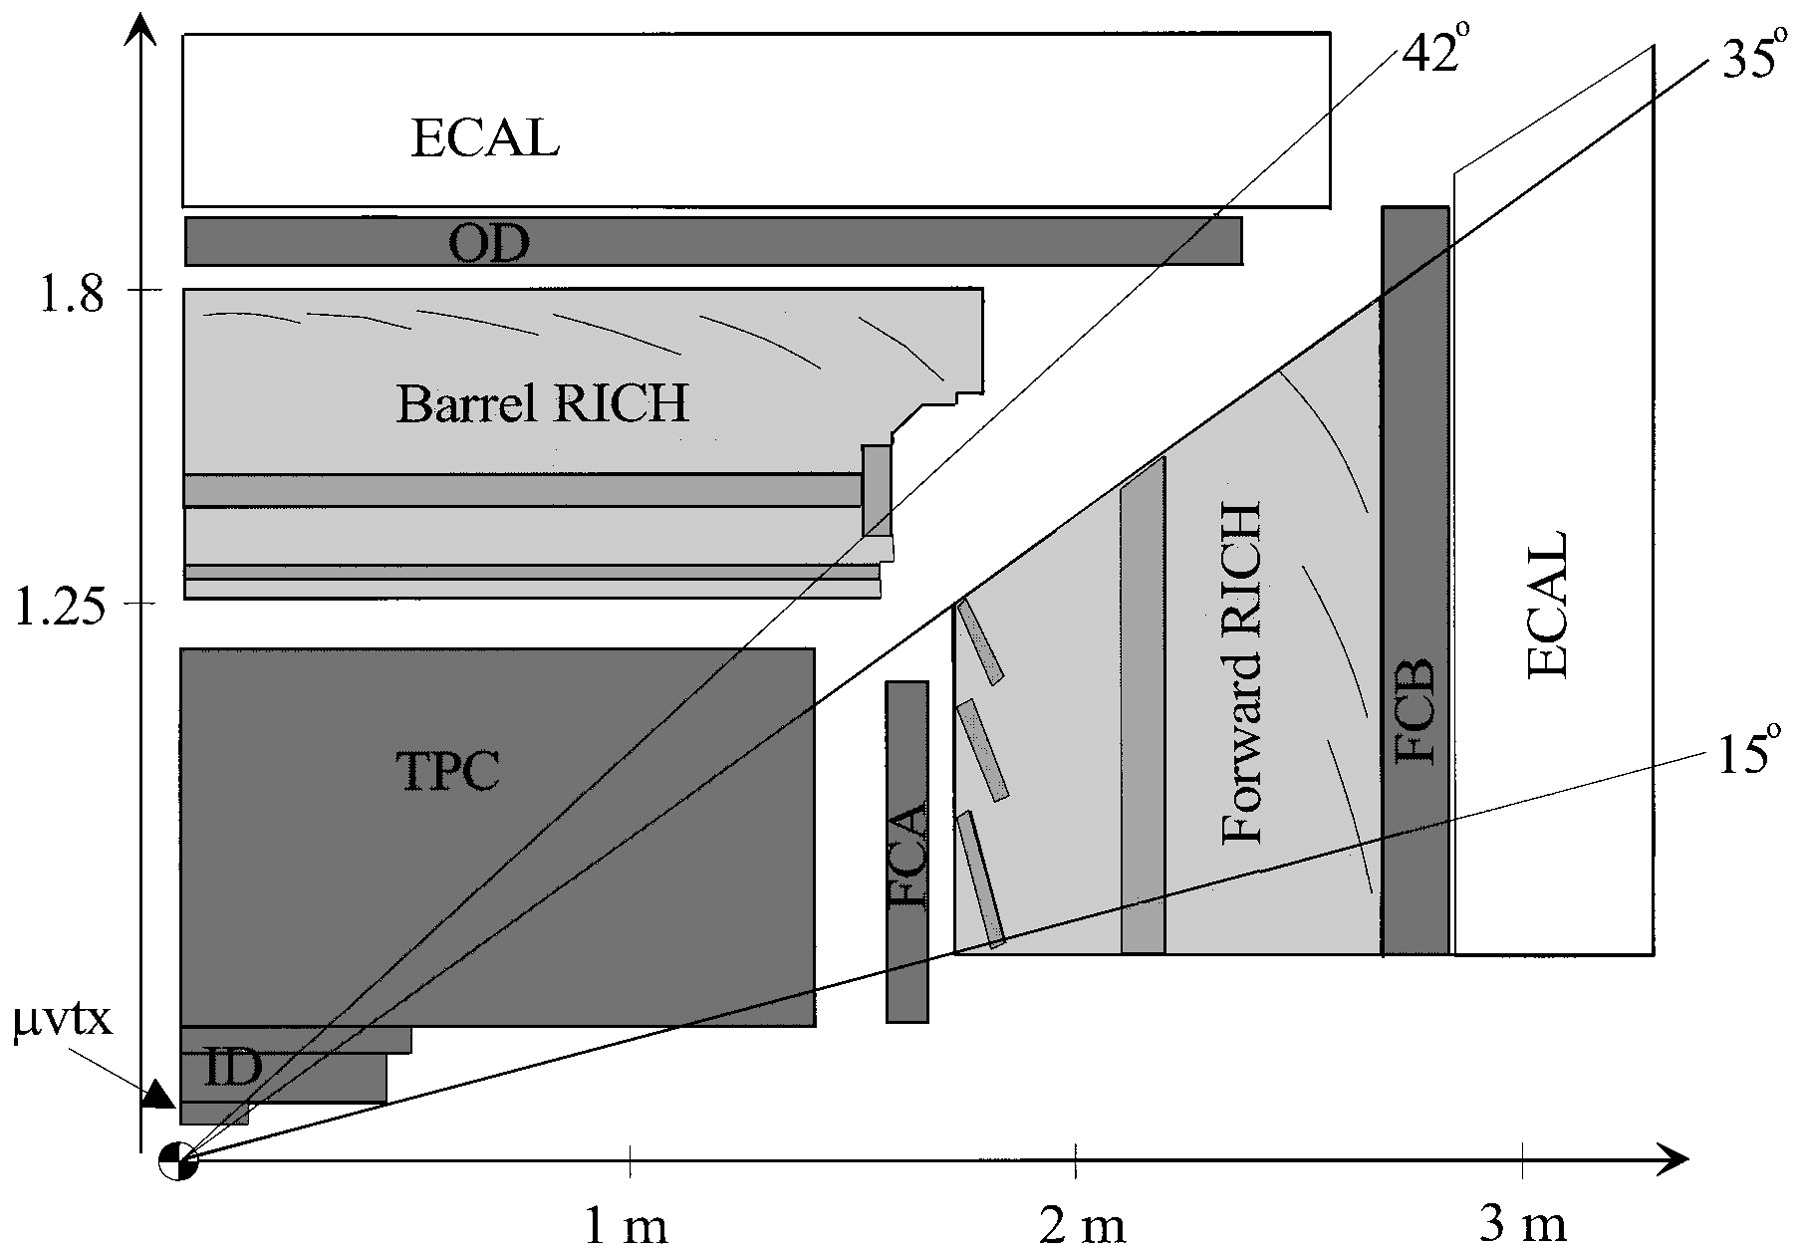
\includegraphics[height = 3.0cm]{Plots/DELPHI_RICH.jpg}
      \caption{DELPHI RICH layout}
    \end{subfigure}%
    \begin{subfigure}{0.35\textwidth}
      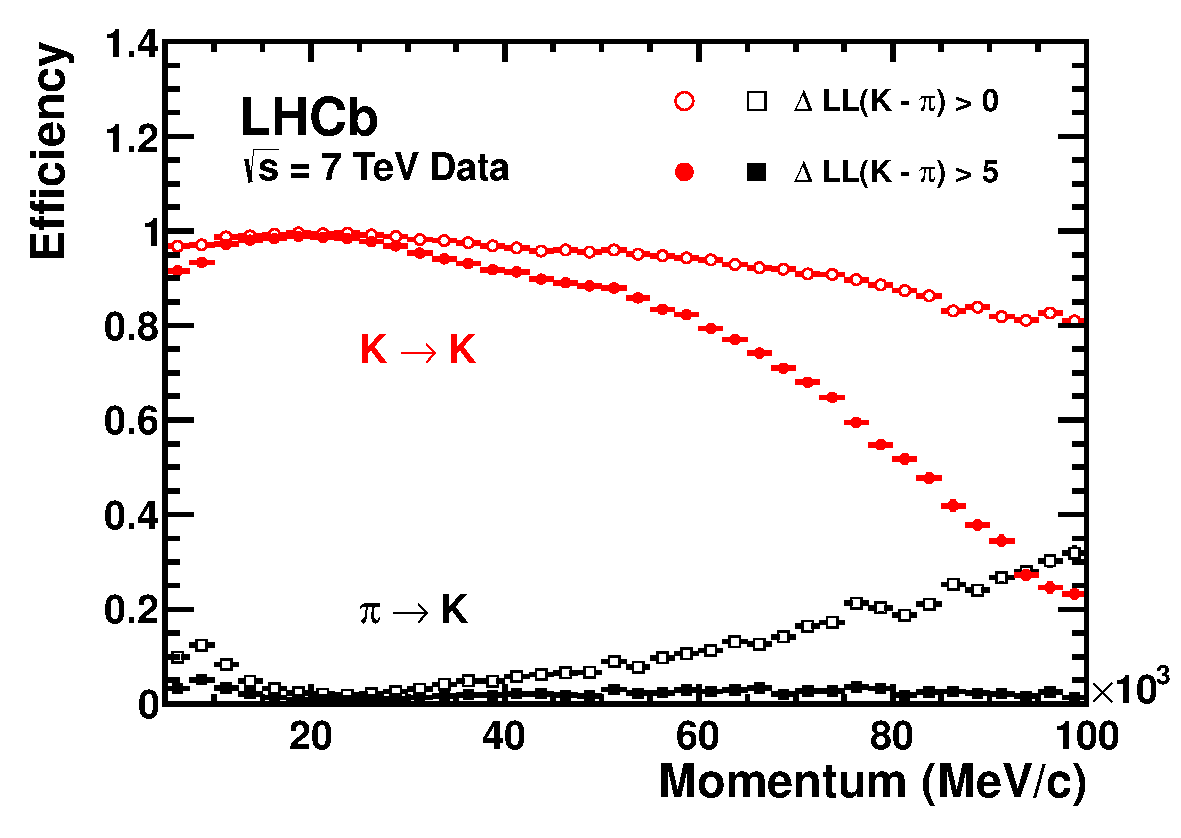
\includegraphics[height = 3.0cm]{Plots/KandPi_2_K.pdf}
      \caption{LHCb RICH performance}
    \end{subfigure}%
    \begin{subfigure}{0.3\textwidth}
      \vspace{-1cm}
      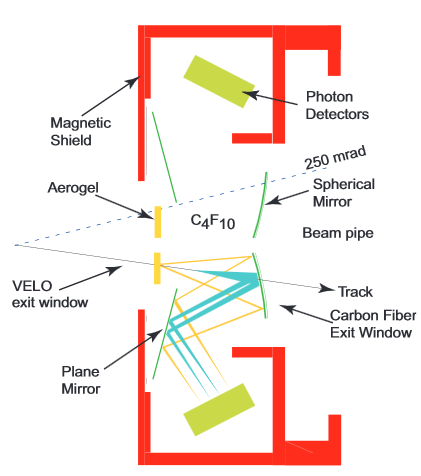
\includegraphics[height = 4.0cm]{Plots/LHCb_RICH.png}
      \caption{LHCb RICH layout}
    \end{subfigure}
  \end{figure}
\end{frame}

\section{Motivation for RICH at FCC-ee}
\begin{frame}{Motivation for RICH at FCC-ee}
  \begin{itemize}
    \setlength\itemsep{0.7em}
    \item{FCC-ee will collect $5\times 10^{12}$ $Z$ boson decays in $4$ years}
    \begin{itemize}
      \item{Allows for a world-leading flavour physics programme}
      \item{Combined with excellent PID capabilities, FCC-ee will reach an unprecedented precision}
    \end{itemize}
    \item{Good PID performance is also required for Higgs, $WW$ and $t\bar{t}$ physics}
    \begin{itemize}
      \item{In particular, kaon ID is crucial for $H\to s\bar{s}$}
    \end{itemize}
  \end{itemize}
  \begin{figure}
    \centering
    \vspace{-0.2cm}
    \begin{subfigure}{0.5\textwidth}
      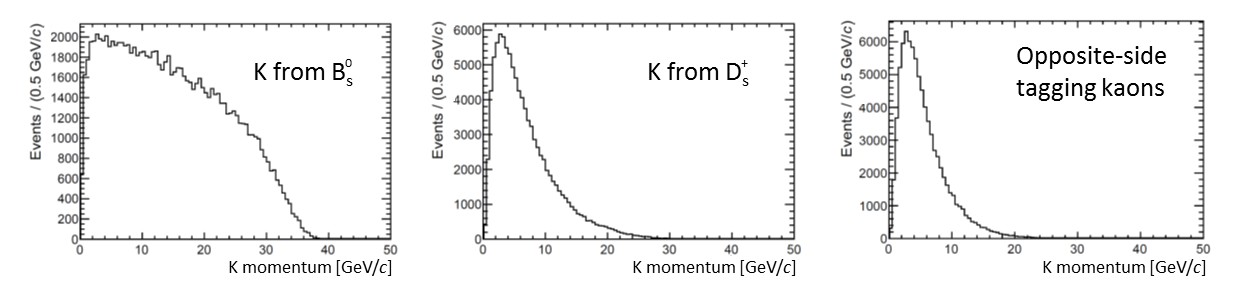
\includegraphics[height = 4cm, trim = {0 0 22.5cm 0}, clip = true]{Plots/p_spectrum_crop.png}
    \end{subfigure}%
    \begin{subfigure}{0.5\textwidth}
      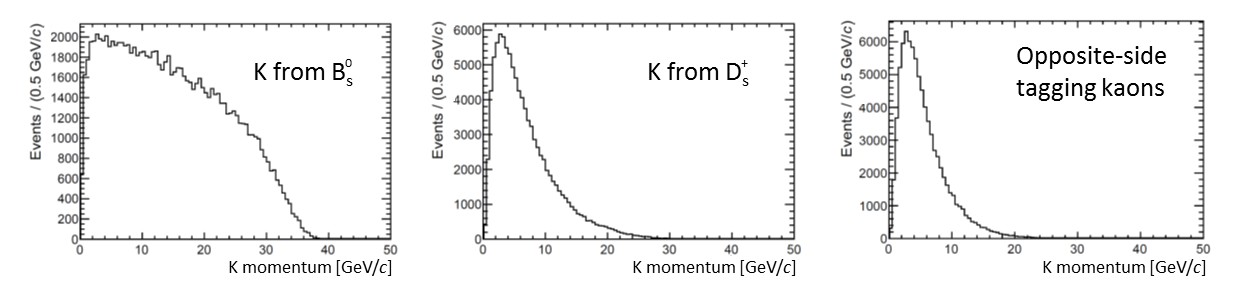
\includegraphics[height = 4cm, trim = {22.0cm 0 0 0}, clip = true]{Plots/p_spectrum_crop.png}
    \end{subfigure}
    \caption{$B_s^0\to D_s^\pm K^\mp$\\$B$ physics requires pion-kaon separation from low momentum up to $\SI{40}{\giga\eV}$}
  \end{figure}
\end{frame}

\begin{frame}{Motivation for RICH at FCC-ee}
  \begin{itemize}
    \setlength\itemsep{0.7em}
    \item{FCC-ee will collect $5\times 10^{12}$ $Z$ boson decays in $4$ years}
    \begin{itemize}
      \item{Allows for a world-leading flavour physics programme}
      \item{Combined with excellent PID capabilities, FCC-ee will reach an unprecedented precision}
    \end{itemize}
    \item{Good PID performance is also required for Higgs, $WW$ and $t\bar{t}$ physics}
    \begin{itemize}
      \item{In particular, kaon ID is crucial for $H\to s\bar{s}$}
    \end{itemize}
  \end{itemize}
  \begin{figure}
    \centering
    \vspace{-0.2cm}
    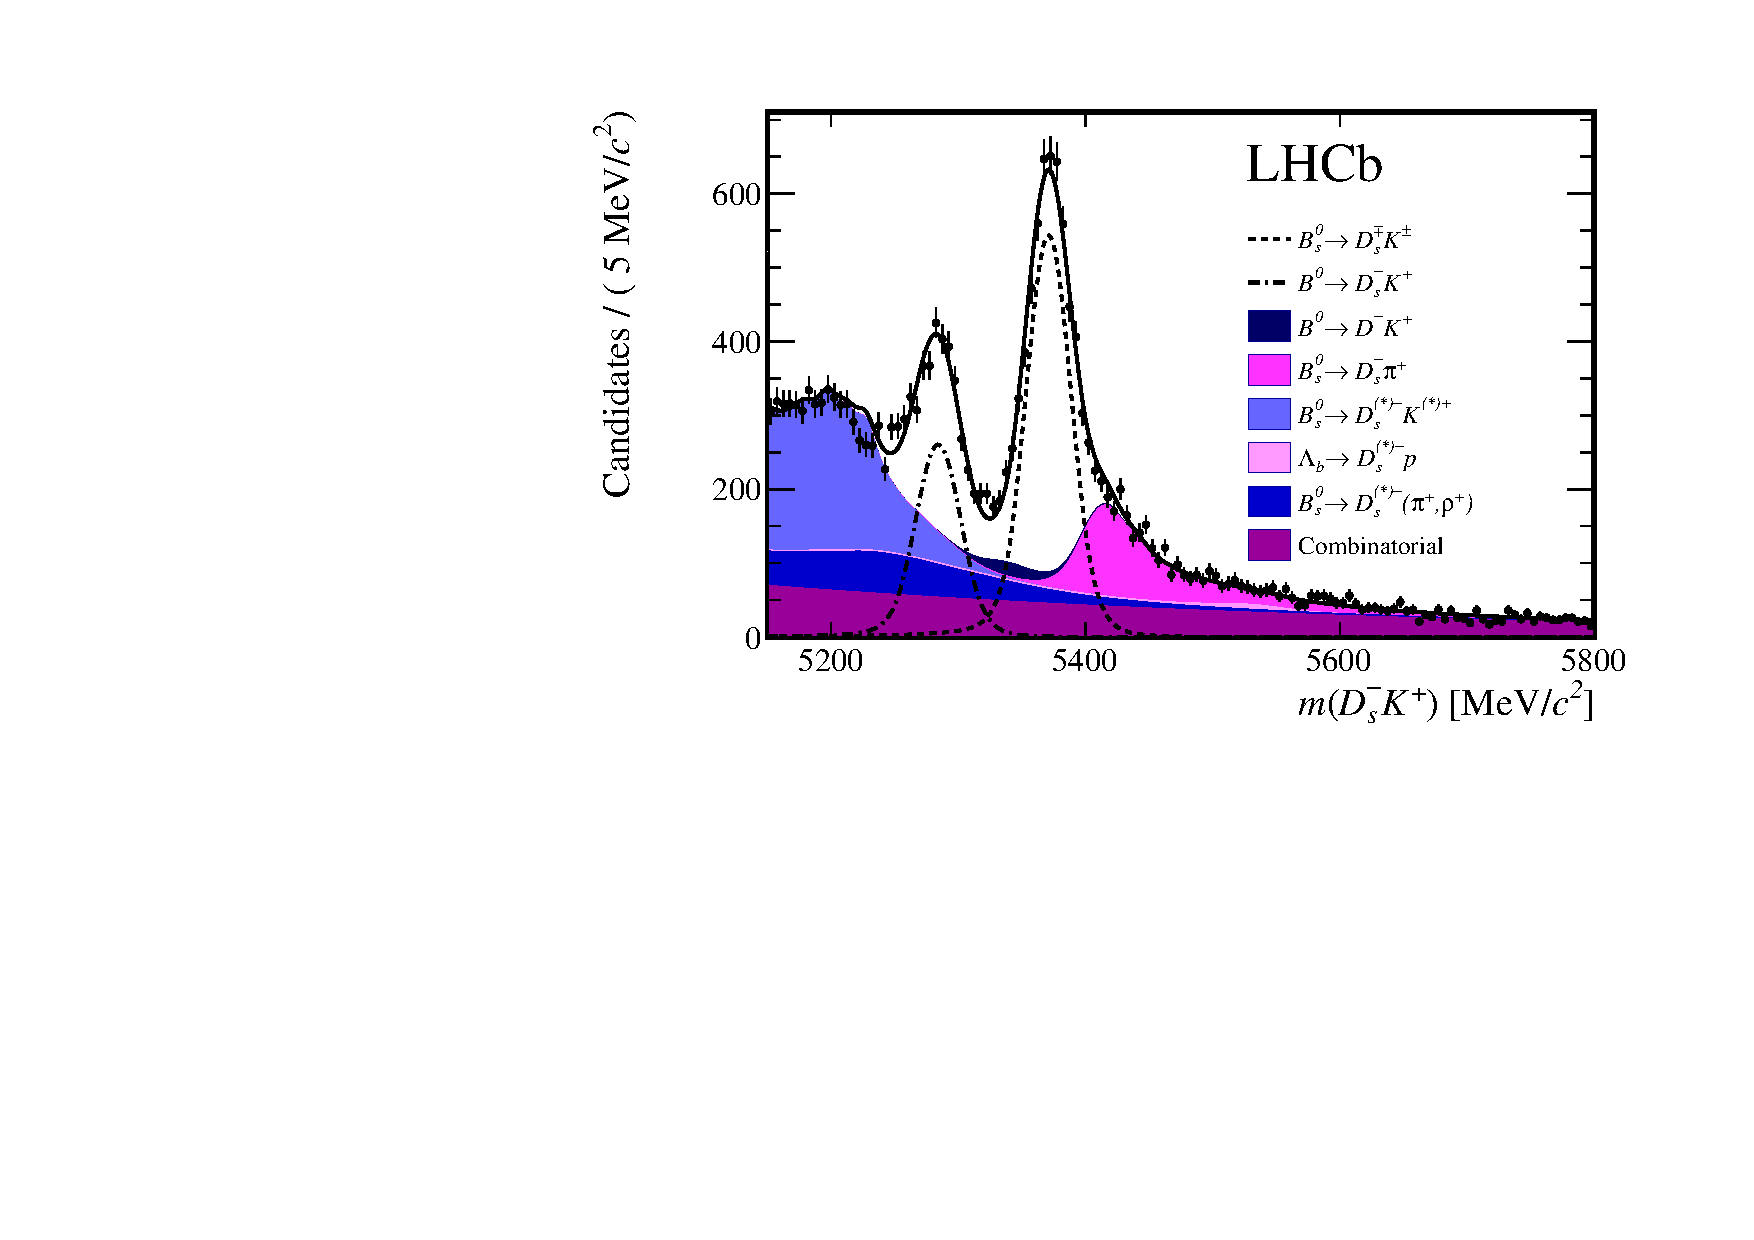
\includegraphics[height = 4cm]{Plots/LHCb_BsDsK.pdf}
    \caption{$B_s^0\to D_s^\pm K^\mp$\\The $B_s^0\to D_s^\pm\pi^\mp$ background would be $10$ times larger without PID capabilities!}
  \end{figure}
\end{frame}

\section{\textbf{A}rray of \textbf{R}ICH \textbf{C}ells}
\begin{frame}{\textbf{A}rray of \textbf{R}ICH \textbf{C}ells}
  \begin{itemize}
    \setlength\itemsep{0.2em}
    \item{\textbf{A}rray of \textbf{R}ICH \textbf{C}ells (ARC): A novel RICH detector concept}
    \begin{itemize}
      \item{First presented by R. Forty at \href{https://indico.cern.ch/event/995850/contributions/4406336/attachments/2274813/3864163/ARC-presentation.pdf}{FCC week 2021}}
      \item{Compact, low-mass solution for particle ID for FCC-ee}
      \item{Concept inspired by the compound eyes of an insect}
    \end{itemize}
    \item{Adapted to fit into the \href{https://arxiv.org/abs/1911.12230}{CLD experiment} concept, taking $10\%$ from the tracker volume}
    \begin{itemize}
      \item{Radial depth of $\SI{20}{\centi\meter}$, radius of $\SI{2.1}{\meter}$ and a length of $\SI{4.4}{\meter}$}
      \item{Aim to keep material budget below $0.1X_0$}
    \end{itemize}
    \item{Aerogel and gas radiators with a spherical mirror}
    \begin{itemize}
      \item{Aerogel also acts as thermal insulation between gas and detector}
    \end{itemize}
  \end{itemize}
  \begin{figure}
    \centering
    \begin{subfigure}{0.4\textwidth}
      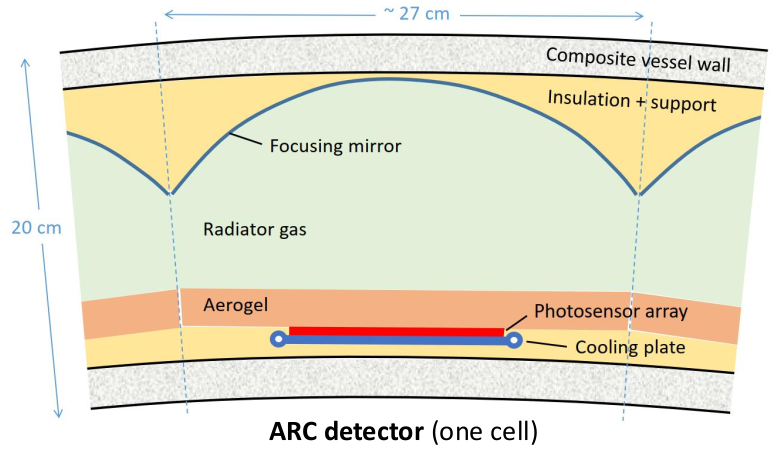
\includegraphics[width = 1.0\textwidth]{Plots/ARC_Cell.png}
    \end{subfigure}%
    \hspace{1cm}
    \begin{subfigure}{0.3\textwidth}
      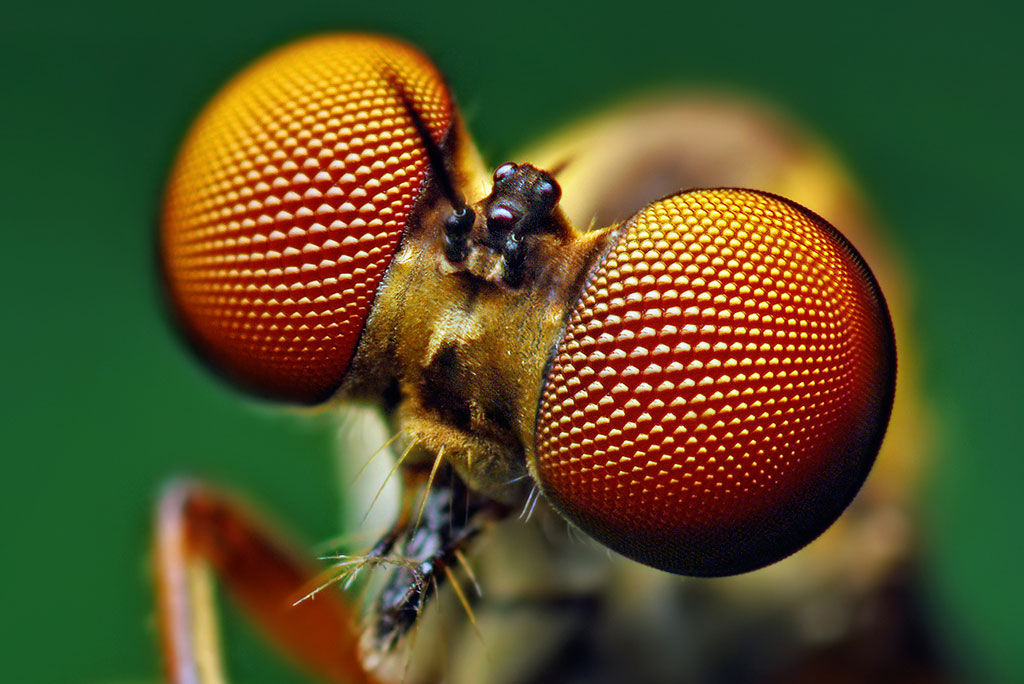
\includegraphics[width = 1.0\textwidth]{Plots/CompoundEyes.jpg}
    \end{subfigure}
    \caption{ARC has a cellular structure, similar to an insect's compound eyes}
  \end{figure}
\end{frame}

\begin{frame}{Original pressurised ARC}
  \begin{itemize}
    \setlength\itemsep{0.5em}
    \item{Original idea was for a vessel with pressurised gas}
    \begin{itemize}
      \item{Higher photon yield in smaller radial space}
    \end{itemize}
    \item{However, a non-pressurised gas was found to have better performance, and also simplify the vessel design}
  \end{itemize}
  \begin{figure}
    \centering
    \begin{subfigure}{0.35\textwidth}
      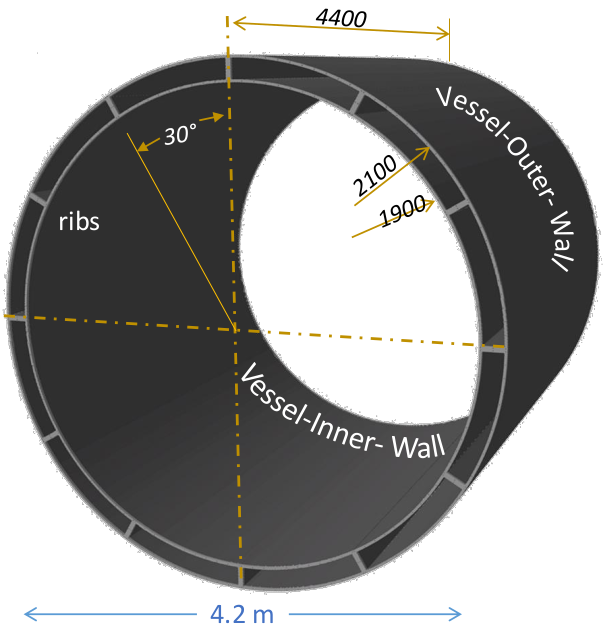
\includegraphics[width = 1.0\textwidth]{Plots/CarbonFiberVessel.png}
    \end{subfigure}%
    \hspace{0.7cm}
    \begin{subfigure}{0.35\textwidth}
      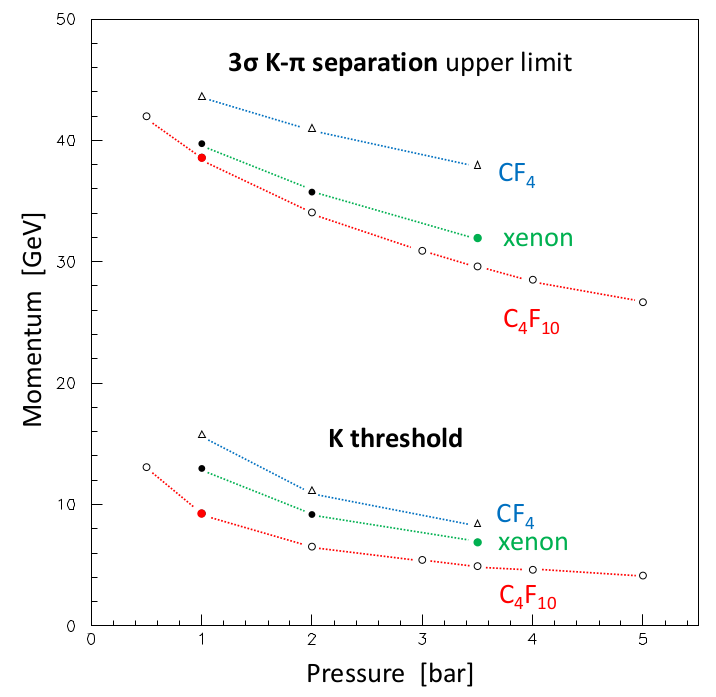
\includegraphics[width = 1.0\textwidth]{Plots/Significance_vs_Pressure.png}
    \end{subfigure}
    \caption{Layout of original carbon fiber vessel (left) and the performance at different pressures (right)}
  \end{figure}
\end{frame}

\begin{frame}{\textbf{A}rray of \textbf{R}ICH \textbf{C}ells}
  \begin{itemize}
    \setlength\itemsep{0.5em}
    \item{Cell layout has evolved to profit from a simplified unpressurised vessel}
    \item{All cells are the same size, organised on a hexagonal grid}
    \begin{itemize}
      \item{Barrel (endcap) has $945$ ($384$) cells in total, where $18$ ($21$) are unique}
      \item{Hexagonal shape avoids the corners, where performance is worse}
    \end{itemize}
  \end{itemize}
  \begin{figure}
    \centering
    \begin{subfigure}{0.6\textwidth}
      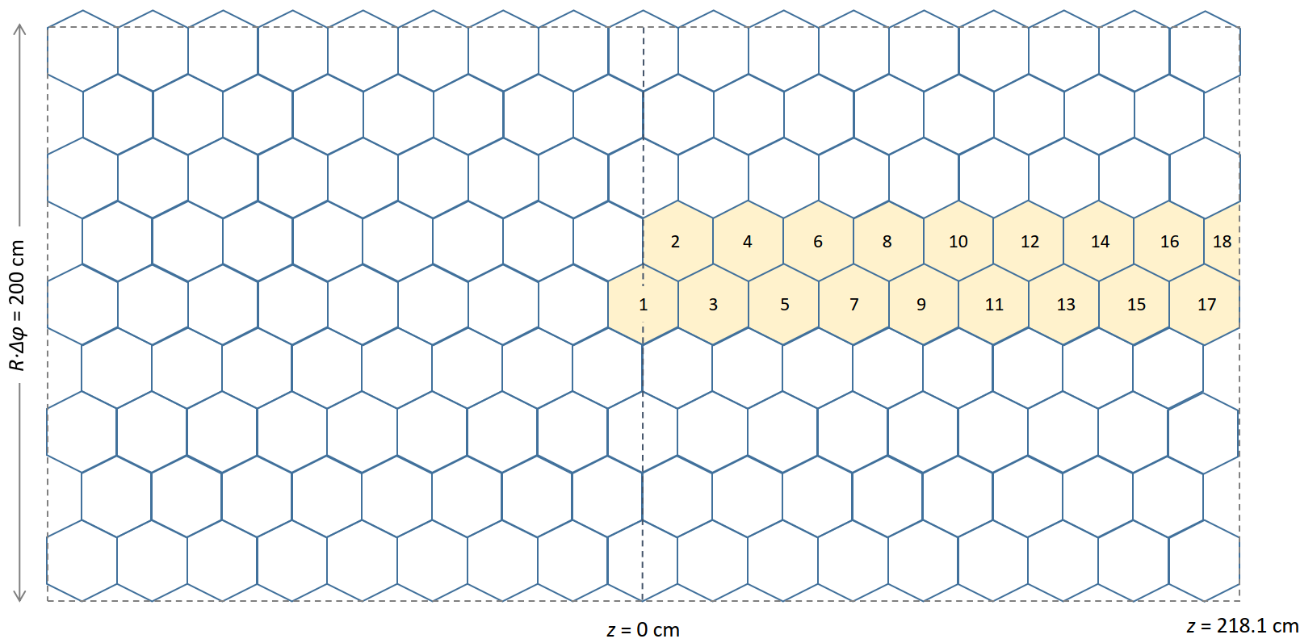
\includegraphics[width = 1.0\textwidth]{Plots/BarrelCells.png}
    \end{subfigure}%
    \begin{subfigure}{0.3\textwidth}
      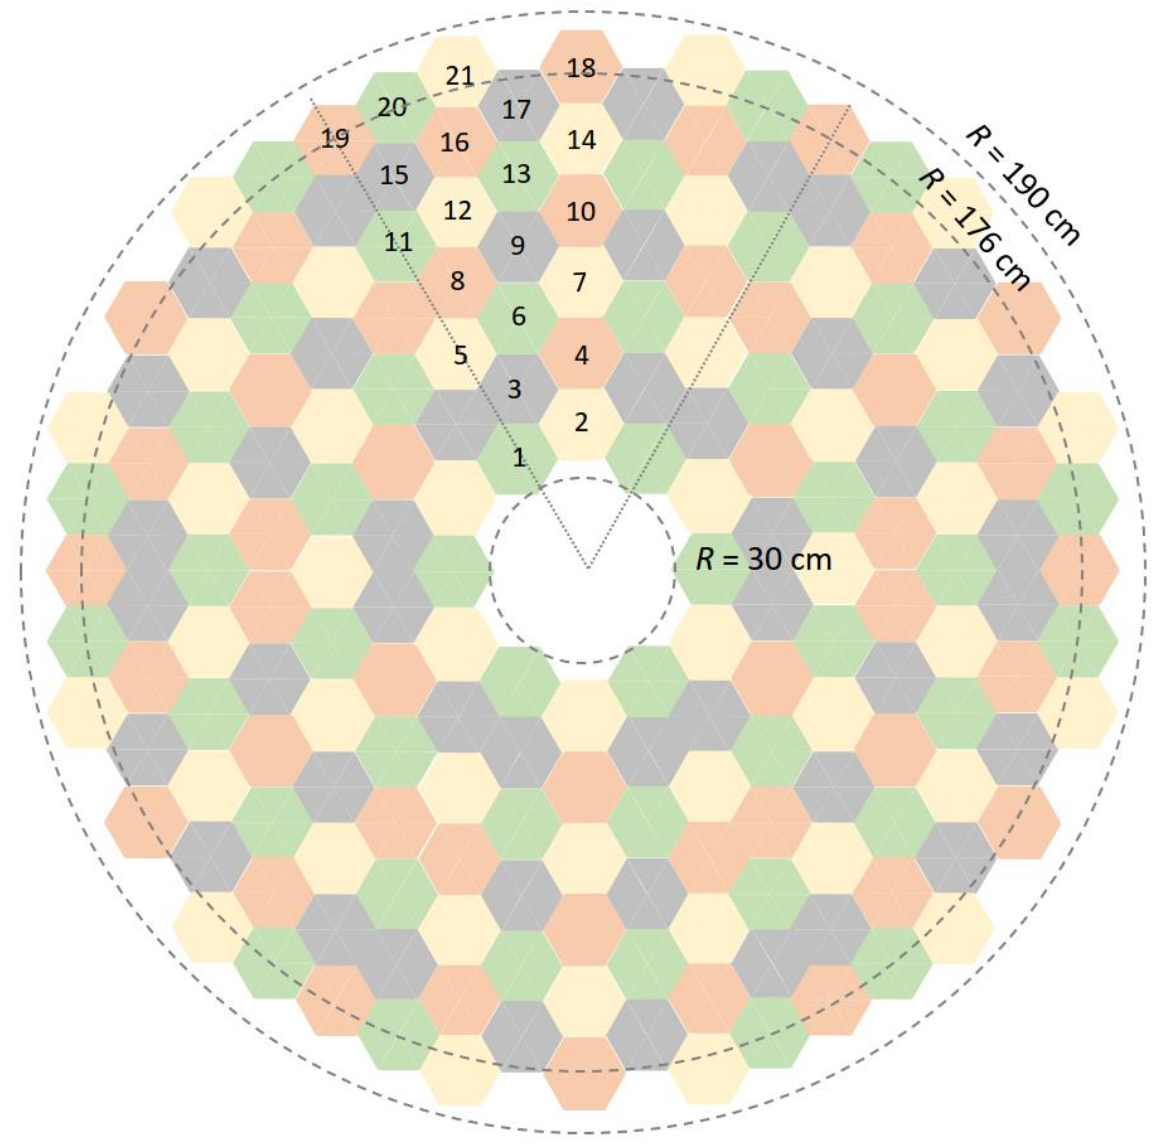
\includegraphics[width = 1.0\textwidth]{Plots/EndcapCells.png}
    \end{subfigure}
    \caption{Barrel (left) and endcap (right) cells}
  \end{figure}
\end{frame}

\section{ARC radiators}
\begin{frame}{ARC radiators}
  \begin{itemize}
    \setlength\itemsep{0.5em}
    \item{$C_4F_{10}$:}
    \begin{itemize}
      \setlength\itemsep{0.2em}
      \item{Baseline assumption, well known from LHCb RICH1}
      \item{$n = 1.0014\implies\theta_c = \SI{53}{\milli\radian}$, suitable for high momentum particles}
      \item{$C_4F_{10}$ is a greenhouse gas, substitution with pressurised Ar/Xe possible}
    \end{itemize}
    \item{Aerogel:}
    \begin{itemize}
      \setlength\itemsep{0.2em}
      \item{Well known as a RICH radiator, e.g. from ARICH at Belle II}
      \item{$n = 1.01$-$1.10\implies\theta_c = 141$-$\SI{430}{\milli\radian}$, suitable at low momentum}
      \item{Very low thermal conductivity}
      \begin{itemize}
        \item{Suitable to separate gas from detector, which must be cooled}
        \item{Cherenkov photons come for ``free'' and are focused by the same mirror}
      \end{itemize}
      \item{Drawback: Some loss of photons from scattering}
    \end{itemize}
  \end{itemize}
  \begin{figure}
    \centering
    \begin{subfigure}{0.25\textwidth}
      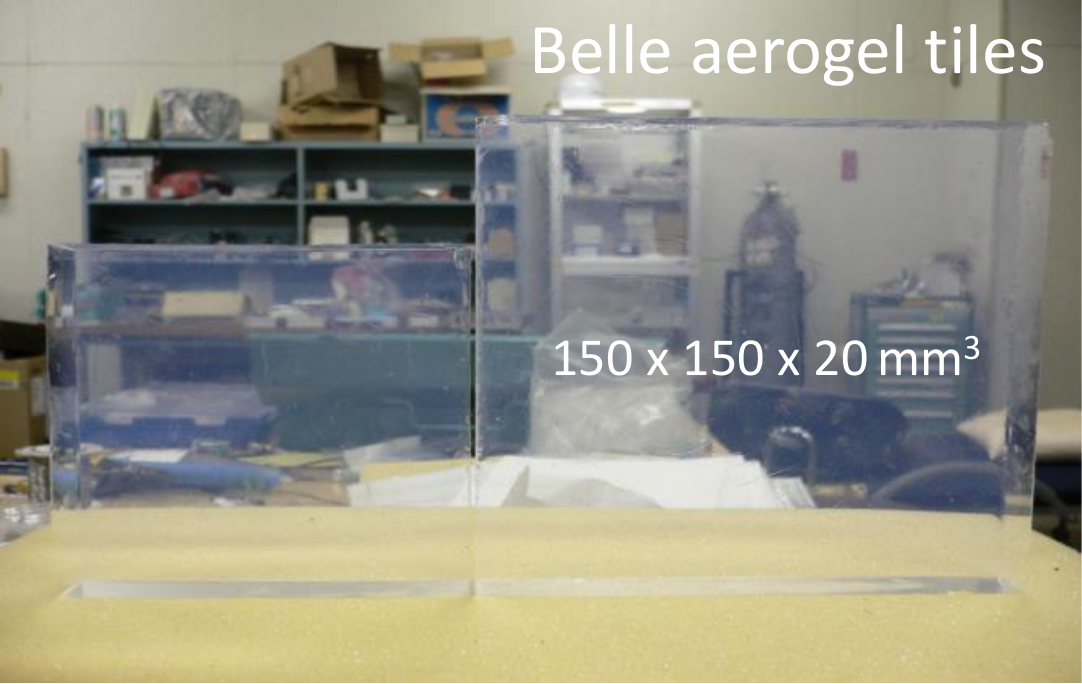
\includegraphics[width = 1.0\textwidth]{Plots/BelleAerogelTiles.png}
    \end{subfigure}%
    \hspace{0.2cm}
    \begin{subfigure}{0.25\textwidth}
      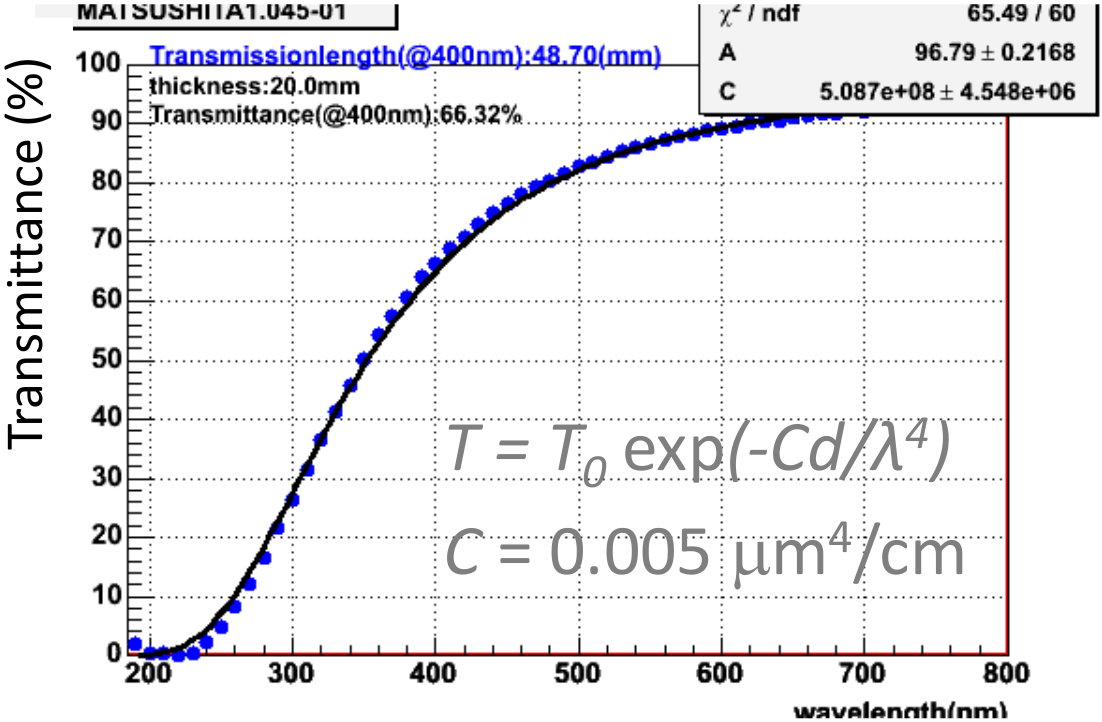
\includegraphics[width = 1.0\textwidth]{Plots/AerogelTransmission.png}
    \end{subfigure}
    \caption{Belle aerogel tiles (left) and aerogel transmission function (right).}
  \end{figure}
\end{frame}

\section{Event displays}
\begin{frame}{Photon hits}
  \begin{figure}
    \centering
    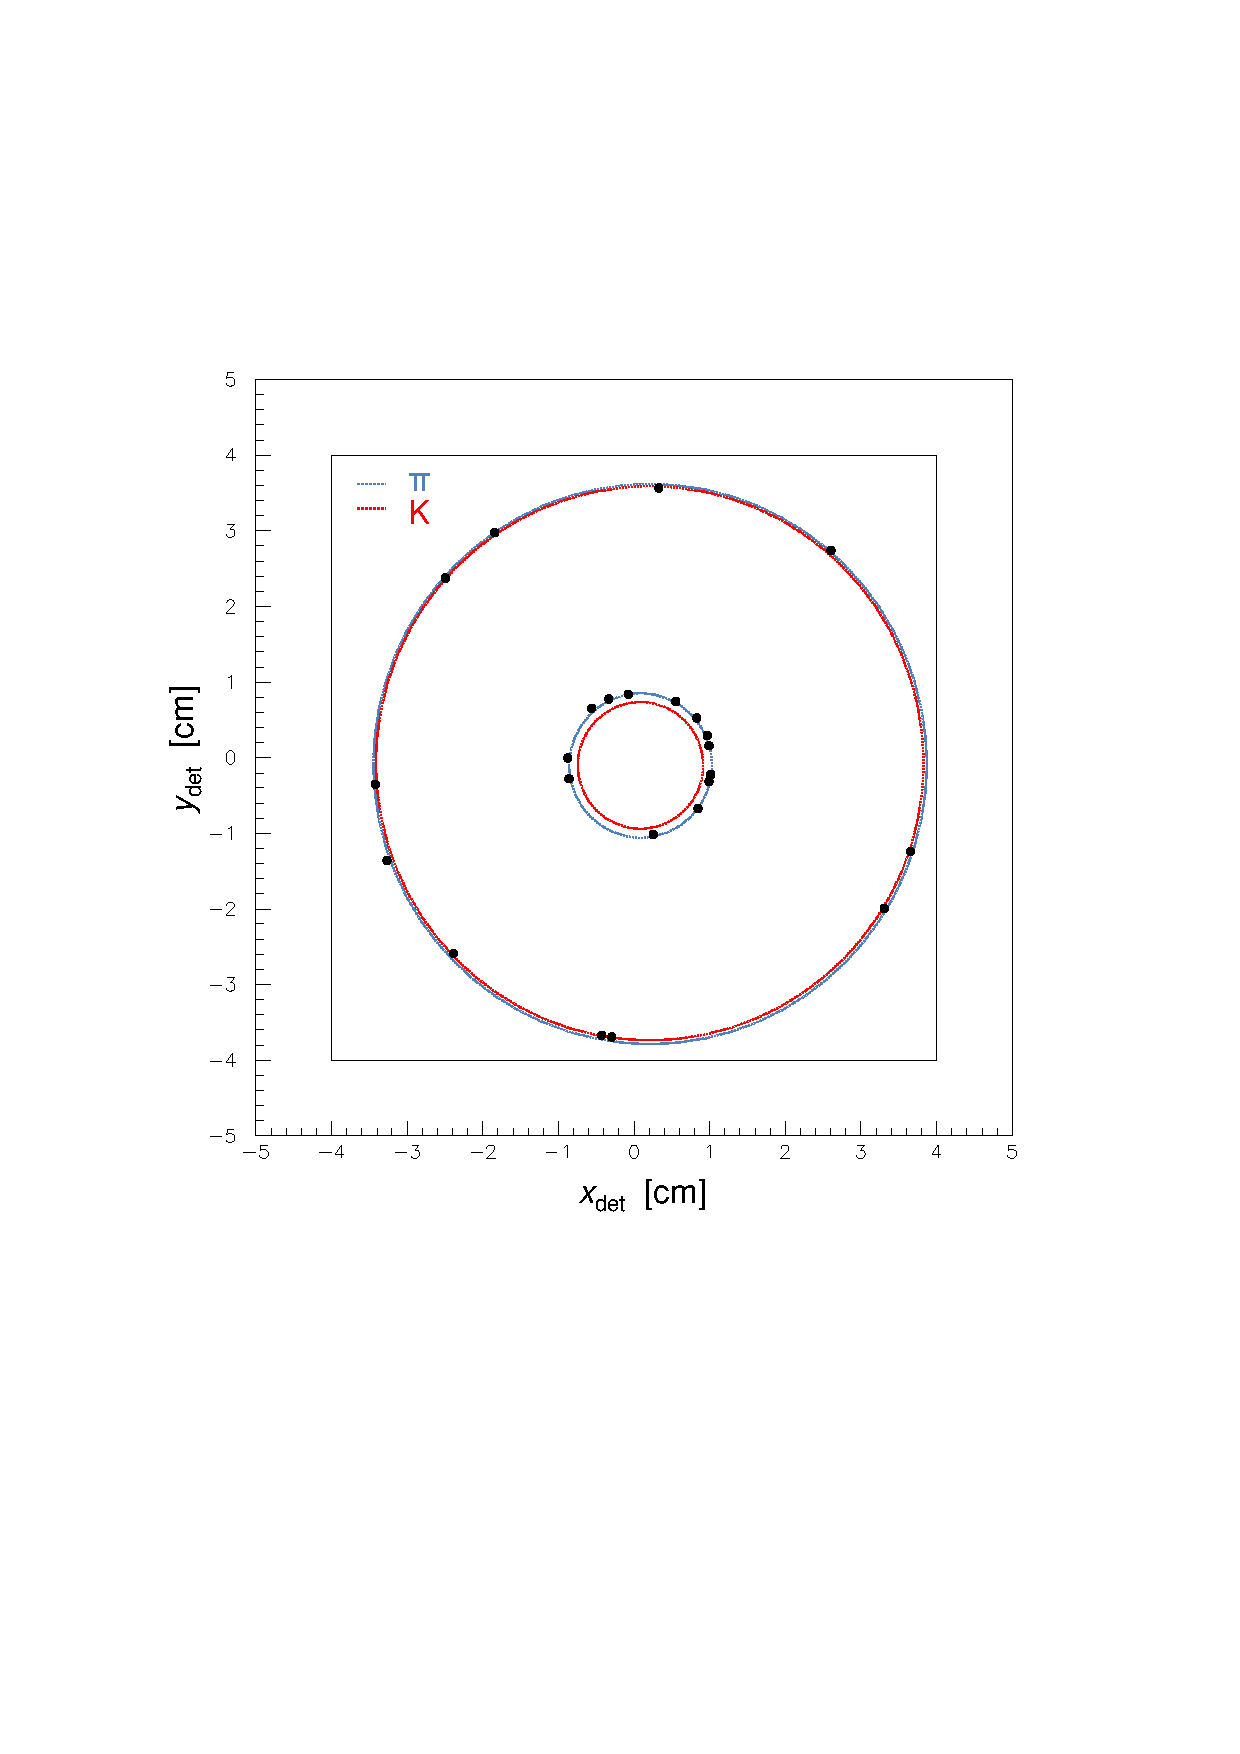
\includegraphics[width = 1.0\textwidth, trim = {4cm 2cm 4cm 2cm}, clip = true]{Plots/Display1.pdf}
    \caption{Photon hits on photodetector}
  \end{figure}
\end{frame}

\begin{frame}{Event display}
  \begin{figure}
    \centering
    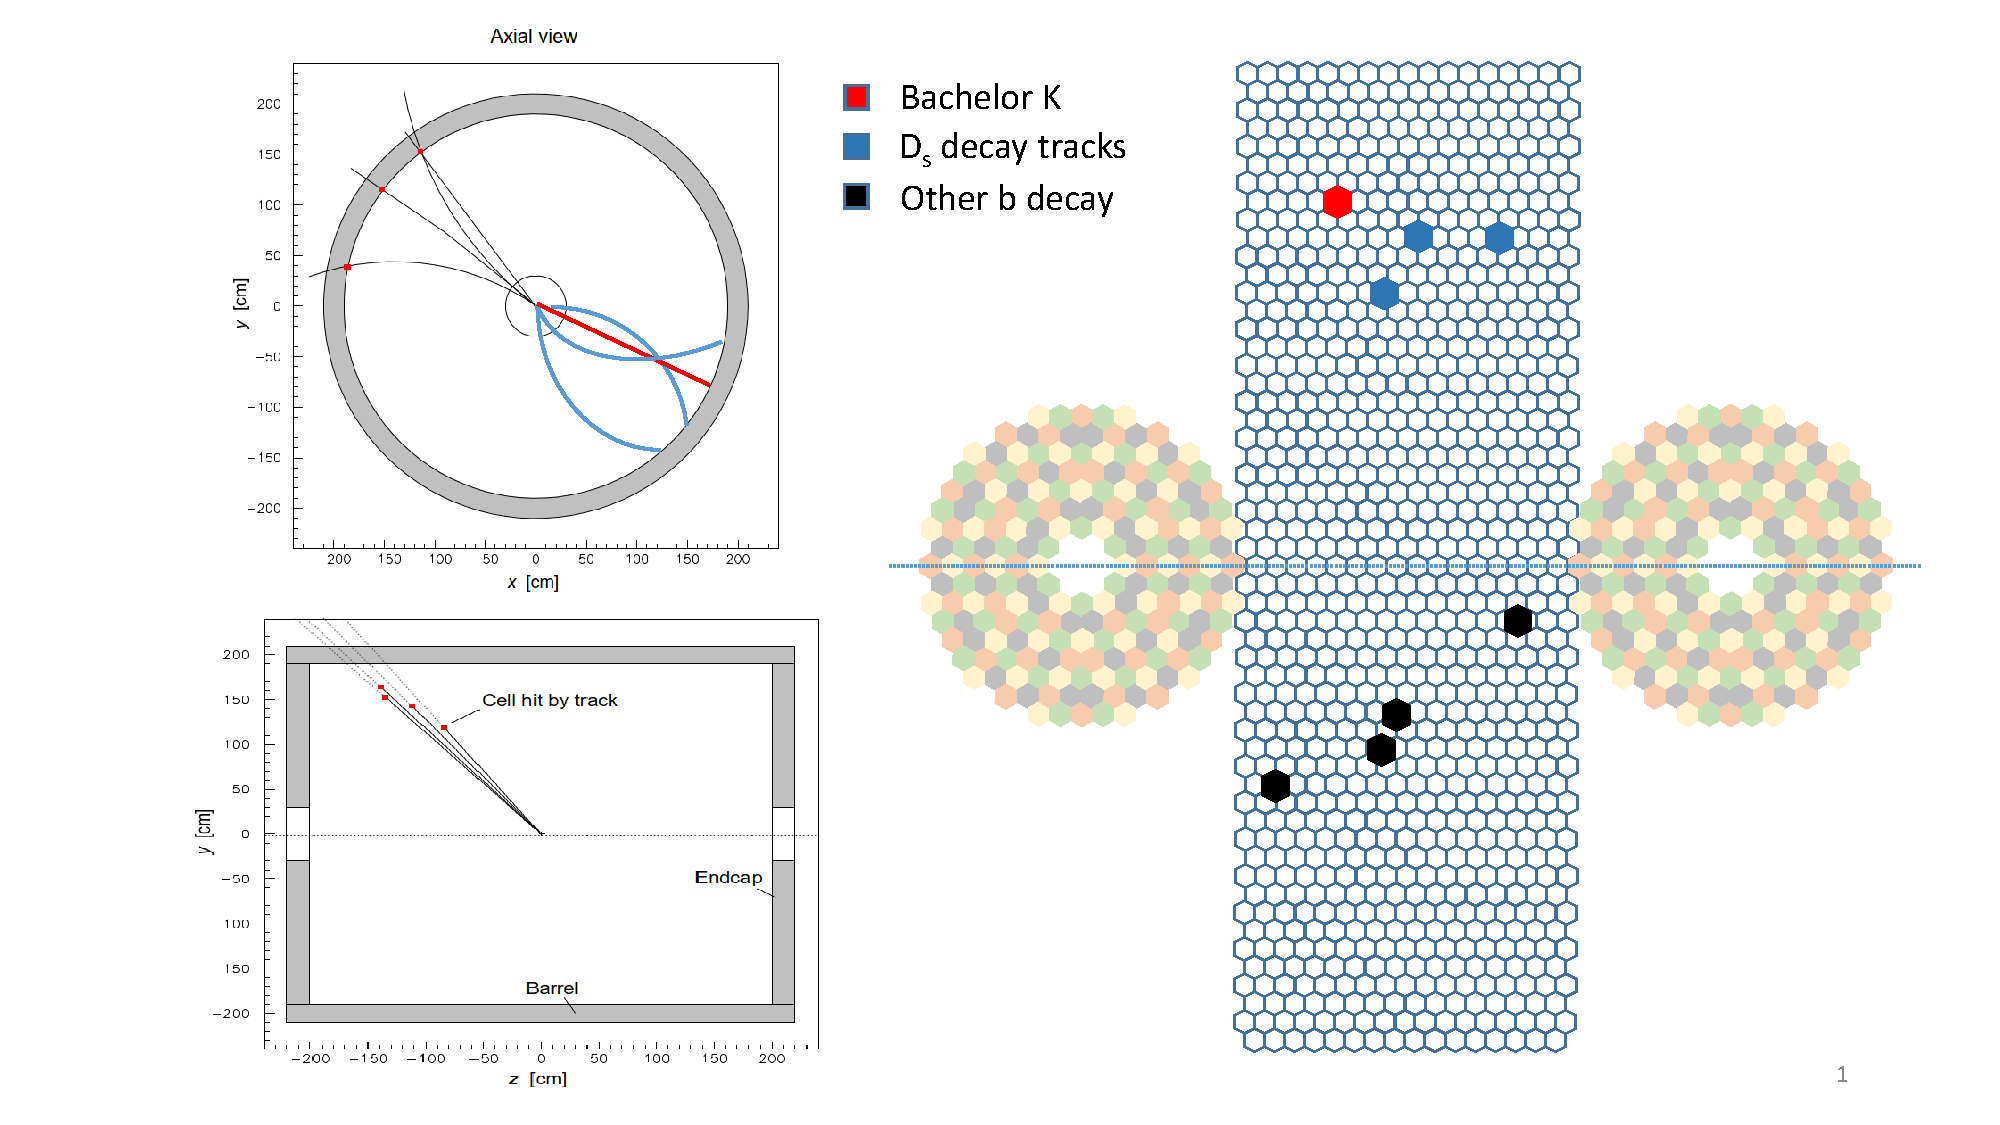
\includegraphics[width = 0.85\textwidth, trim = {0cm 2cm 0cm 0cm}, clip = true]{Plots/Display2.pdf}
    \caption{$B_s\to D_sK$ (no magnetic field yet)}
  \end{figure}
\end{frame}

\section{Optimisation of ARC layout}
\begin{frame}{Optimisation of ARC layout}
  \begin{itemize}
    \setlength\itemsep{0.7em}
    \item{The following procedure is used to evaluate the ARC performance:}
    \begin{enumerate}
      \setlength\itemsep{0.2em}
      \item{Generate straight particle track from IP and trace it through ARC}
      \item{Generate Cherenkov photons from gas radiator}
      \item{Track photons through the optics and to detector}
      \item{Reconstruct Cherenkov angles and calculate standard deviation}
    \end{enumerate}

    \item{Three sources of uncertainty are considered:}
    \begin{enumerate}
      \setlength\itemsep{0.2em}
      \item{Emission point uncertainty: Emission point is assumed to be the mid-point of the track inside the gaseous radiator}
      \item{Chromatic dispersion uncertainty: Spread in Cherenkov angle due to wavelength dependence on refractive index}
      \item{Pixel size: Will be chosen so that it does not limit the performance}
    \end{enumerate}
  \end{itemize}
  \begin{block}{Minimise the Cherenkov angle uncertainty:}
    \begin{equation*}
      \Delta\theta = \frac{1}{\sqrt{N}}\times\frac{1}{1 - N}\times\sum_{i = 0}^{N - 1}(\theta - \bar{\theta})^2
    \end{equation*}
  \end{block}
\end{frame}

\begin{frame}{Examples of photon tracking through optimised layout}
  \begin{figure}
    \centering
    \begin{subfigure}{0.45\textwidth}
      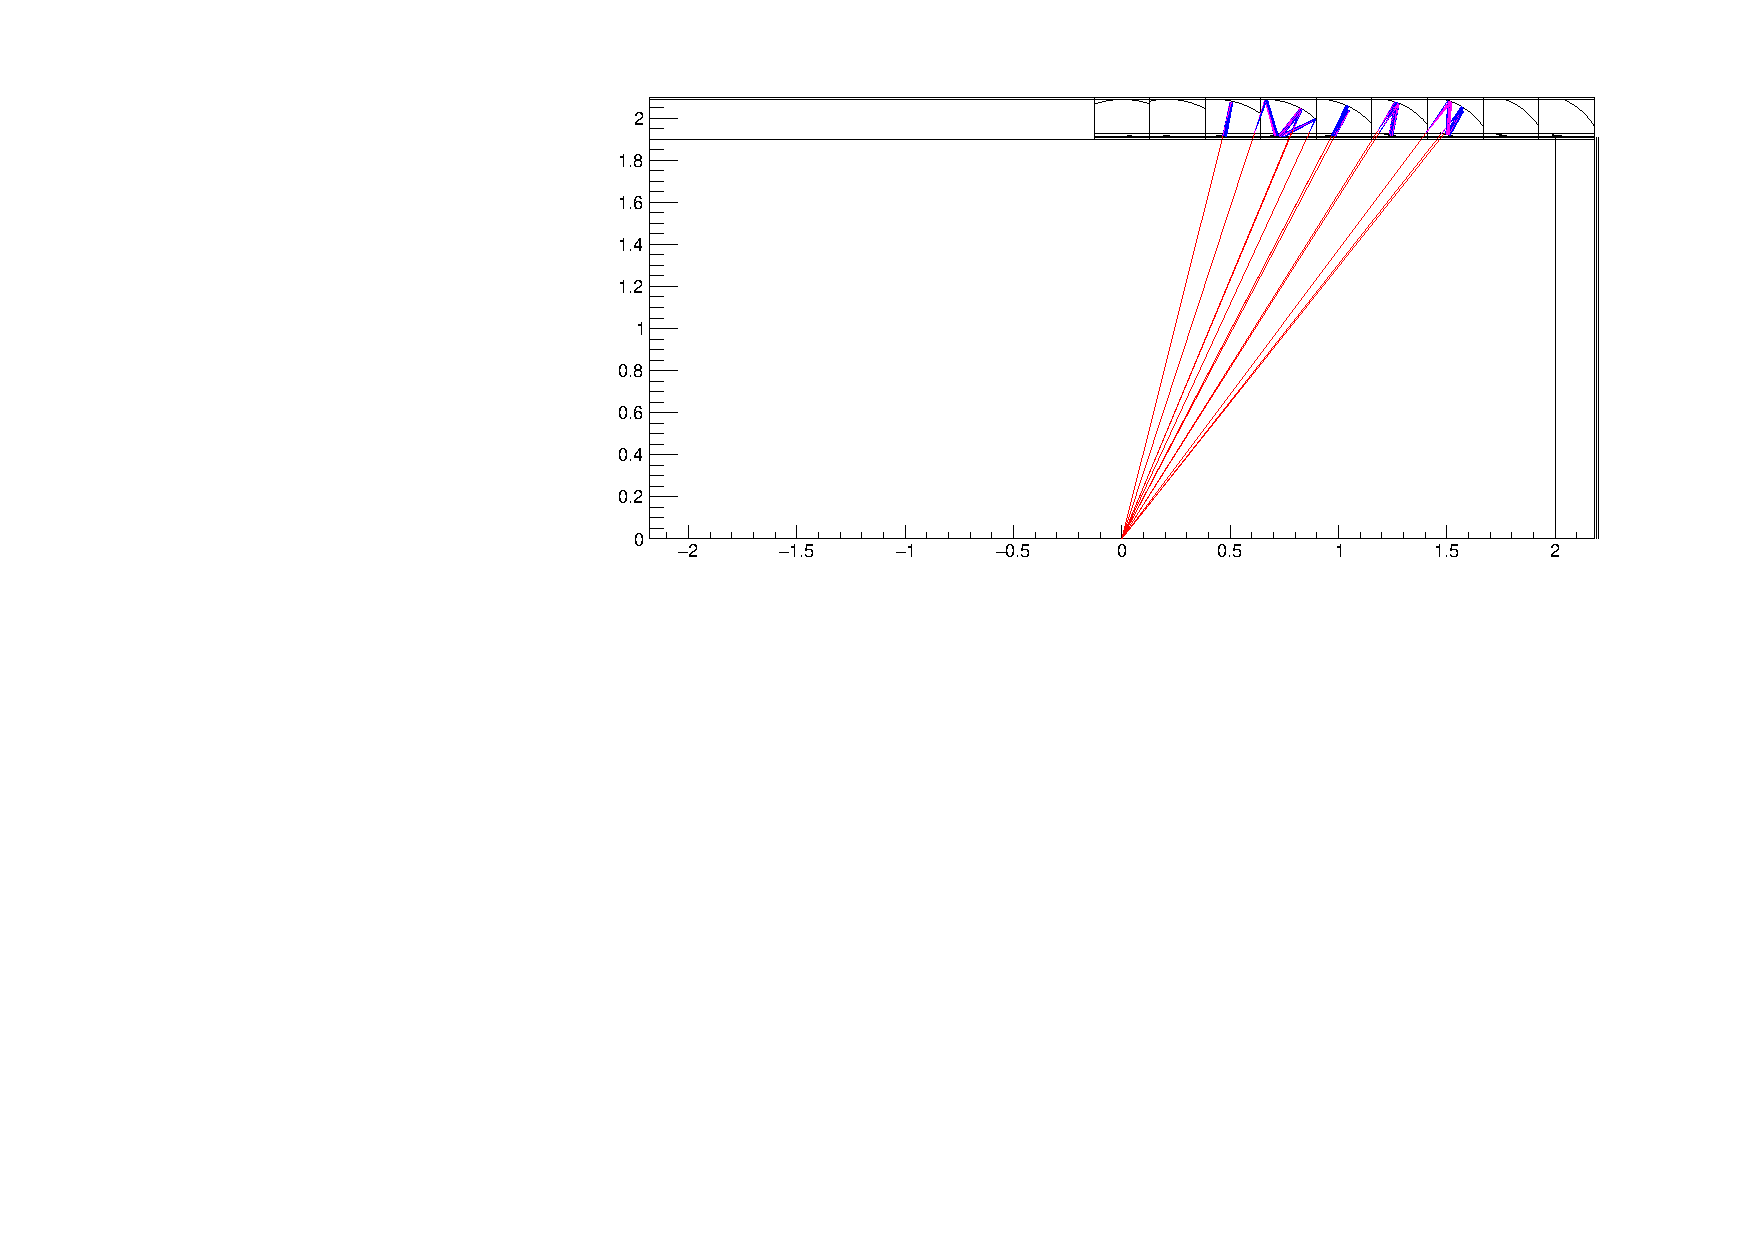
\includegraphics[width = 1.0\textwidth, trim = {11cm 5cm 3.5cm 0}, clip = true]{Plots/EventDisplay_MainRow.pdf}
    \end{subfigure}%
    \hspace{0.2cm}
    \begin{subfigure}{0.45\textwidth}
      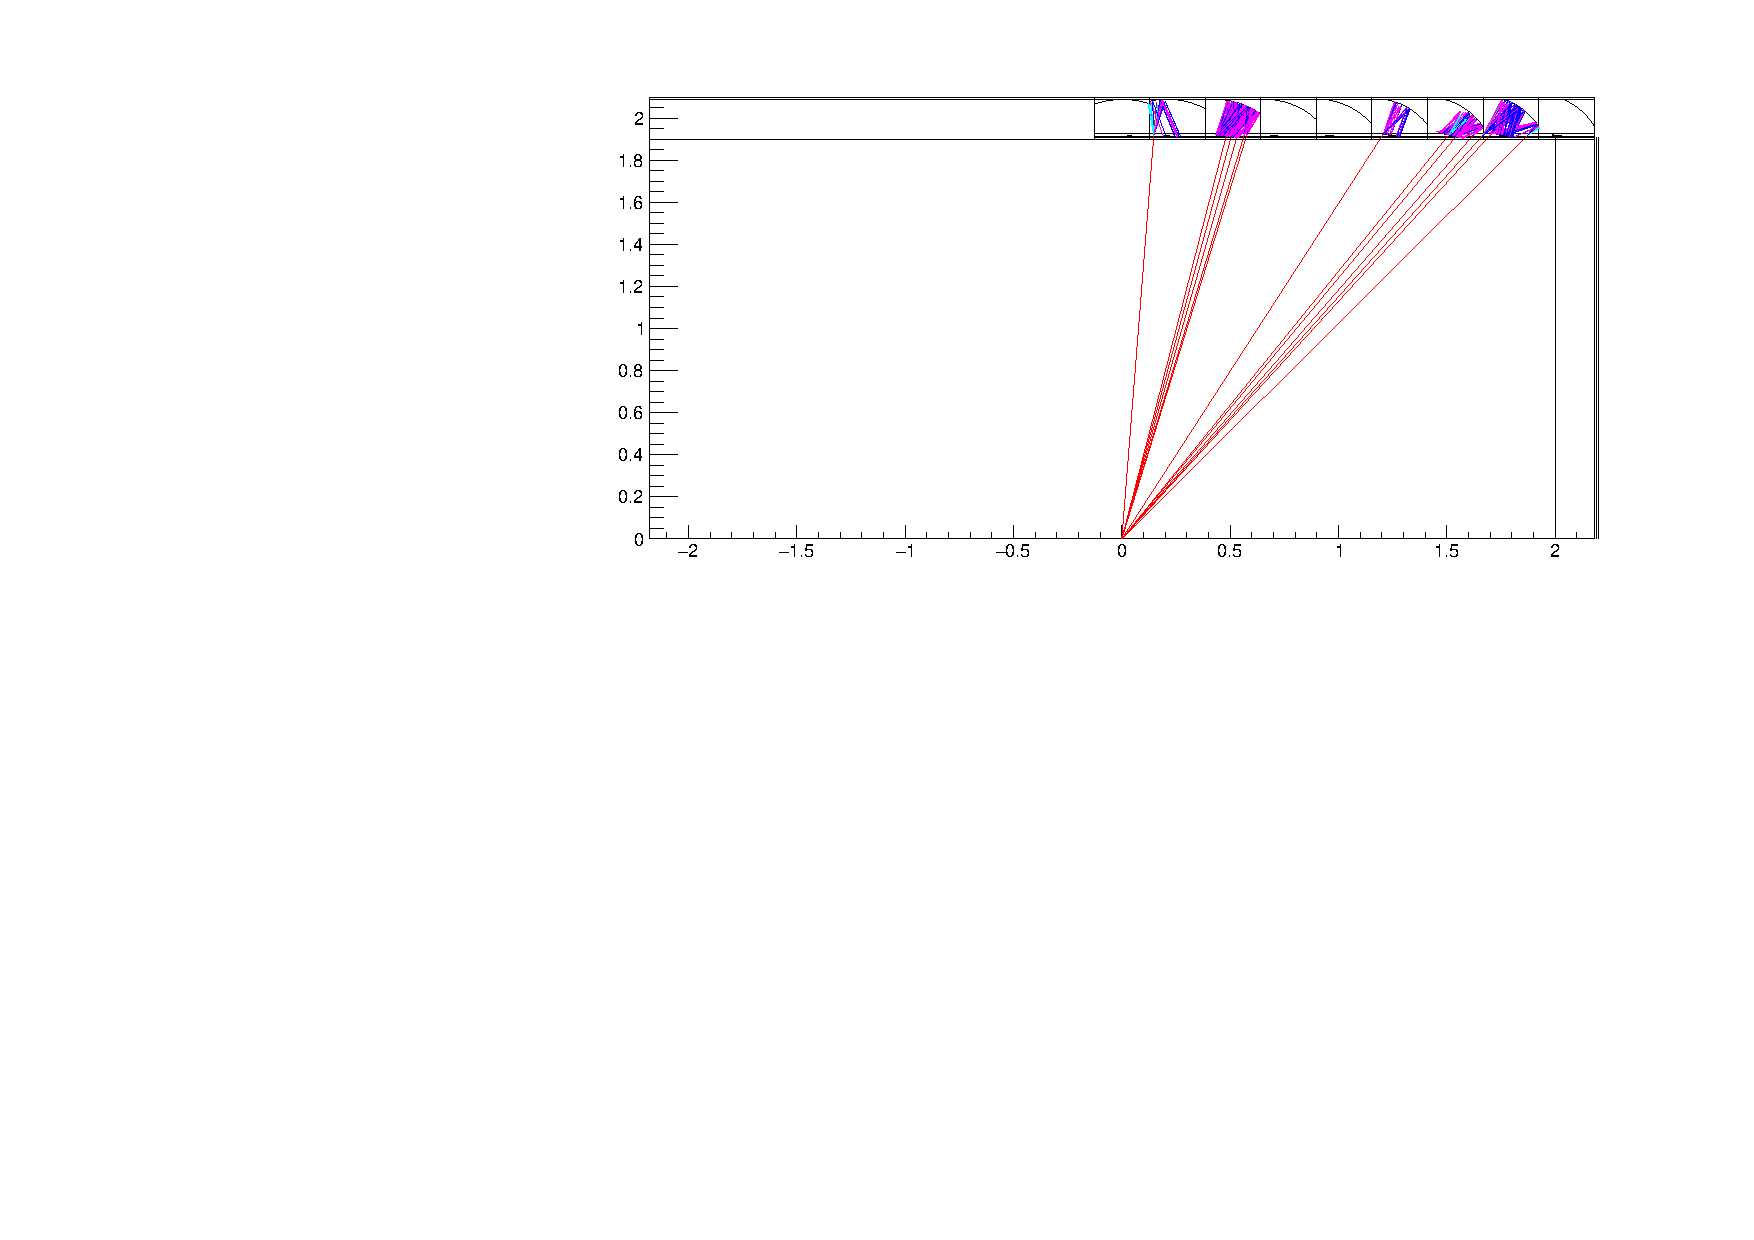
\includegraphics[width = 1.0\textwidth, trim = {11.6cm 5cm 2.9cm 0}, clip = true]{Plots/EventDisplay_MainRow_Aerogel.pdf}
    \end{subfigure}
    \caption{Tracking of photons from gas radiator (left) and aerogel radiator (right) through the ARC optics}
  \end{figure}
  \vspace{-0.3cm}
  \begin{itemize}
    \item{Parameters that are optimised:}
    \begin{itemize}
      \item{Mirror curvature}
      \item{Mirror vertical and horizontal position}
      \item{Detector horizontal position and tilt}
    \end{itemize}
  \end{itemize}
\end{frame}

\begin{frame}{Cherenkov angle uncertainty for gas radiator}
  \begin{figure}
    \centering
    \vspace{-0.2cm}
    \begin{subfigure}{0.35\textwidth}
      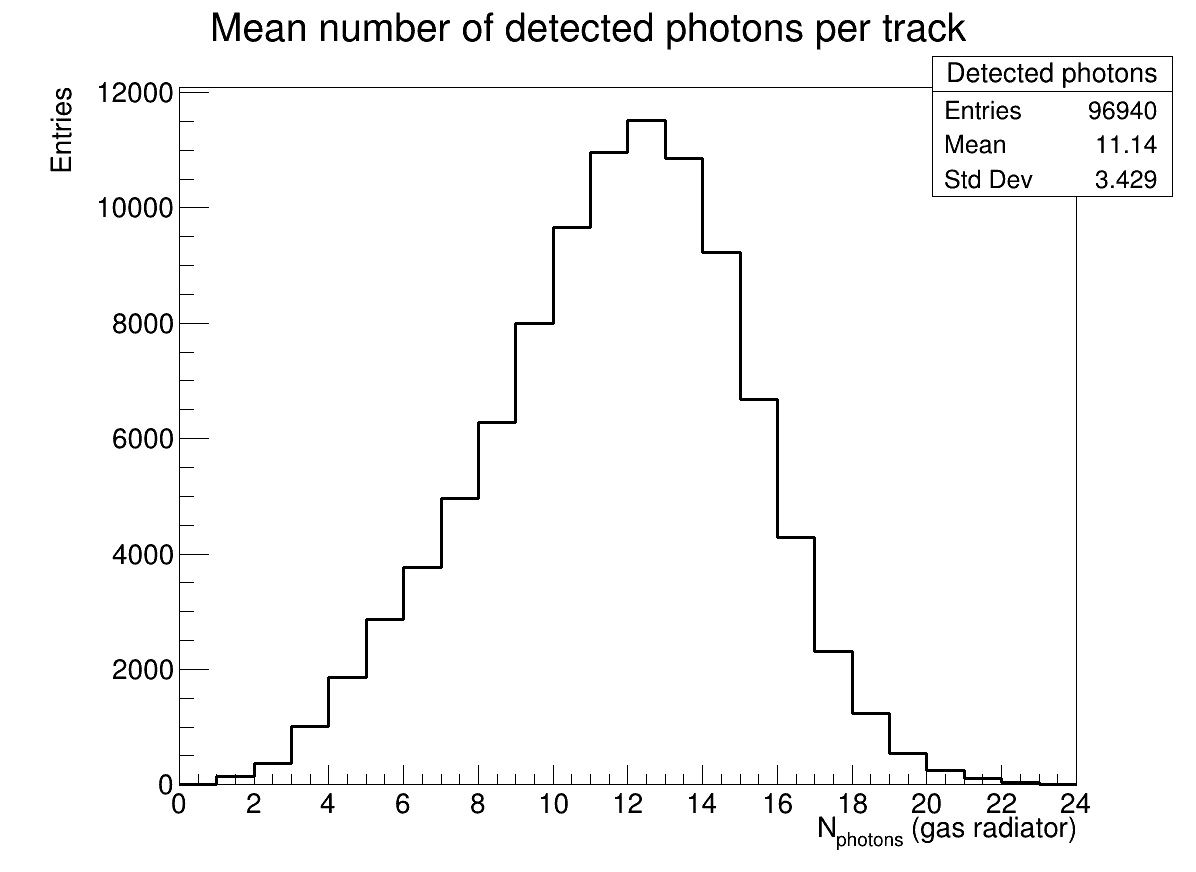
\includegraphics[width = 1.0\textwidth]{Plots/NumberDetectedPhotons_Barrel_Gas.png}
      \vspace{-0.75cm}
      \caption{Mean number of photons detected}
    \end{subfigure}
    \begin{subfigure}{0.35\textwidth}
      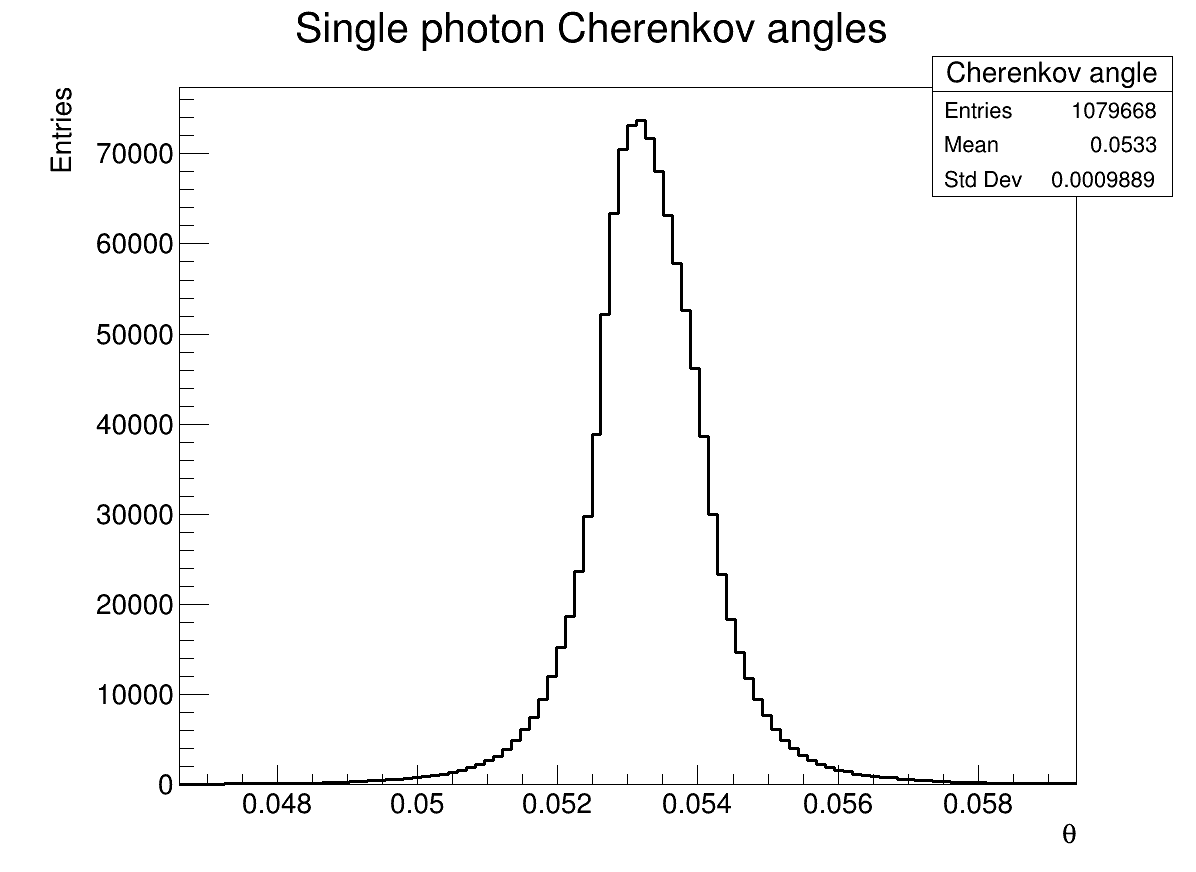
\includegraphics[width = 1.0\textwidth]{Plots/SinglePhotonCherenkovAngles_Barrel_Gas.png}
      \vspace{-0.75cm}
      \caption{Single photon uncertainty:\\ $\SI{1.0}{\milli\radian}$}
    \end{subfigure}%
    \begin{subfigure}{0.35\textwidth}
      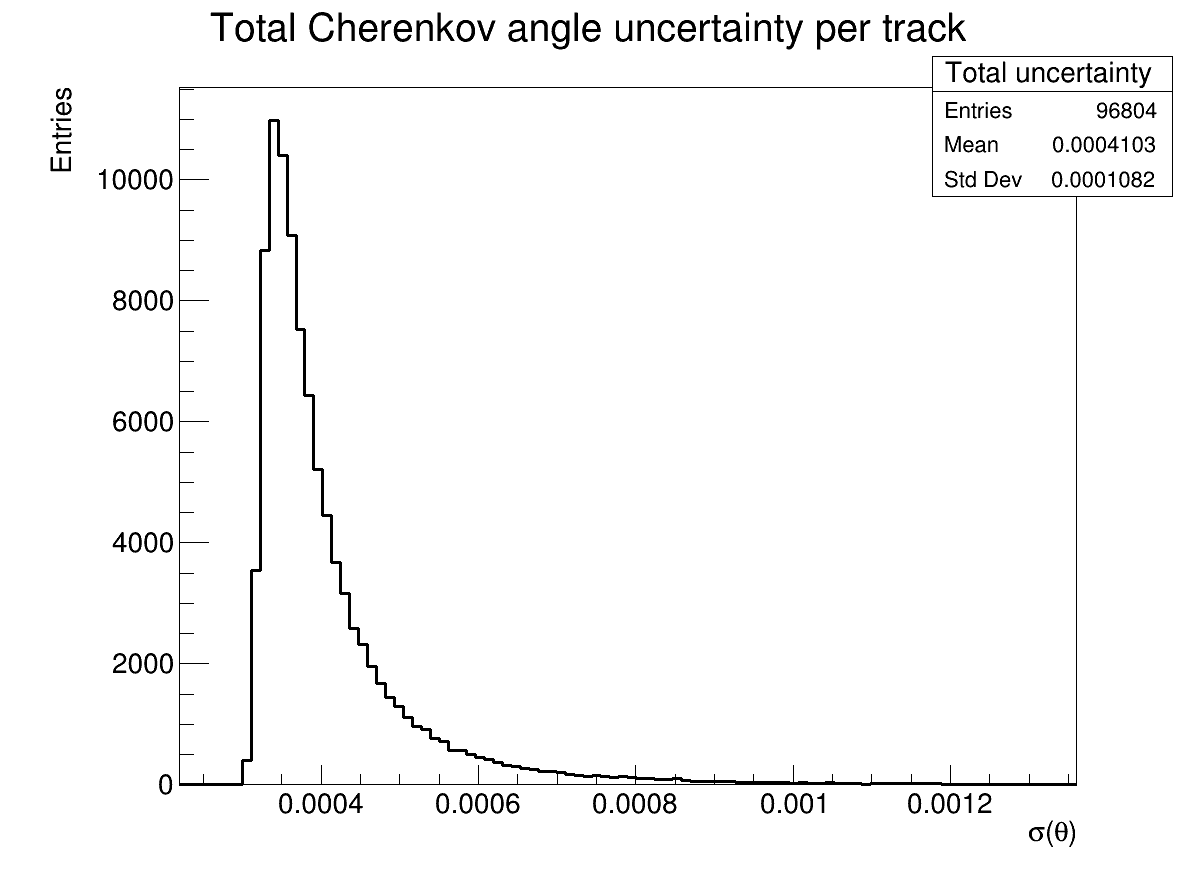
\includegraphics[width = 1.0\textwidth]{Plots/TotalCherenkovUncertainty_Barrel_Gas.png}
      \vspace{-0.75cm}
      \caption{Total uncertainty:\\ $\SI{0.4}{\milli\radian}$}
    \end{subfigure}
    \vspace{-0.1cm}
    \caption{Gas radiator performance averaged over all barrel cells}
  \end{figure}
\end{frame}

\begin{frame}{Cherenkov angle uncertainty for aerogel radiator}
  \begin{figure}
    \centering
    \vspace{-0.2cm}
    \begin{subfigure}{0.35\textwidth}
      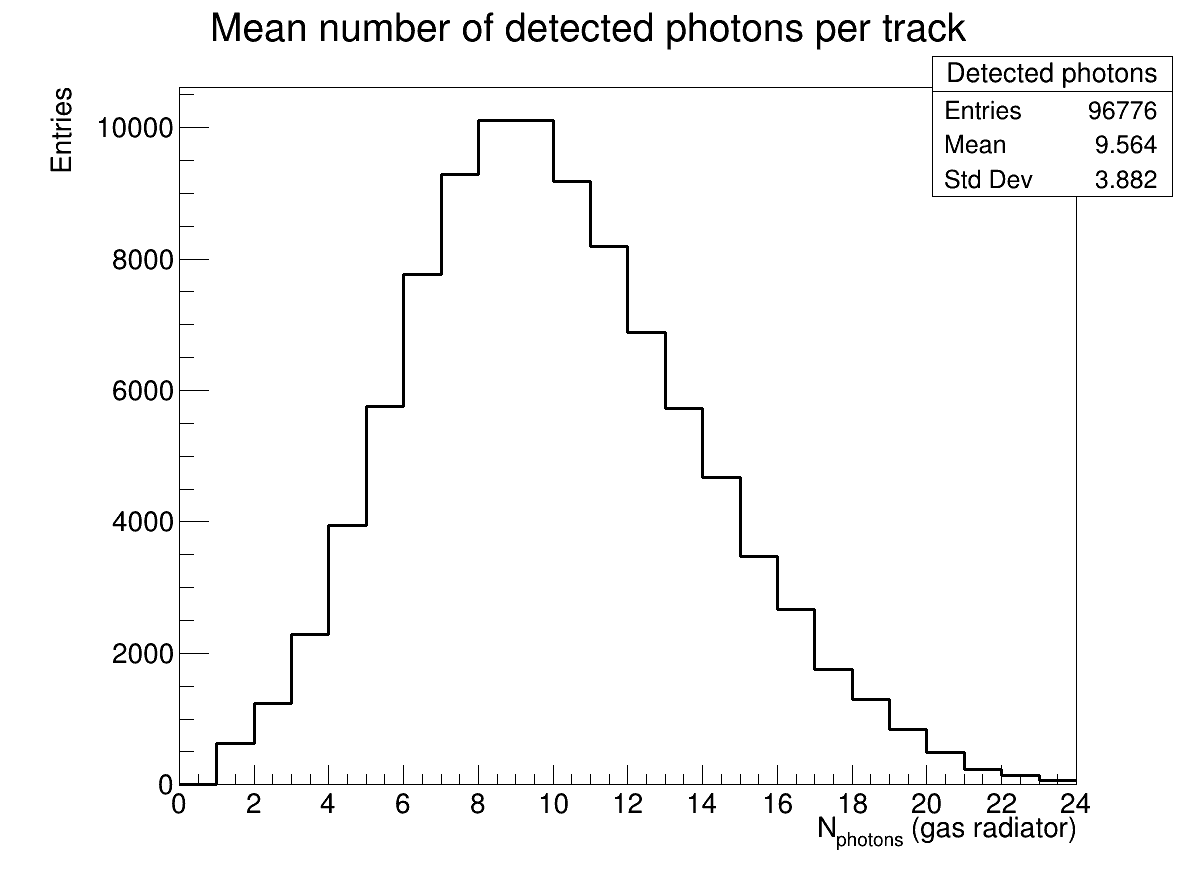
\includegraphics[width = 1.0\textwidth]{Plots/NumberDetectedPhotons_Barrel_Aerogel.png}
      \vspace{-0.75cm}
      \caption{Mean number of photons detected}
    \end{subfigure}
    \begin{subfigure}{0.35\textwidth}
      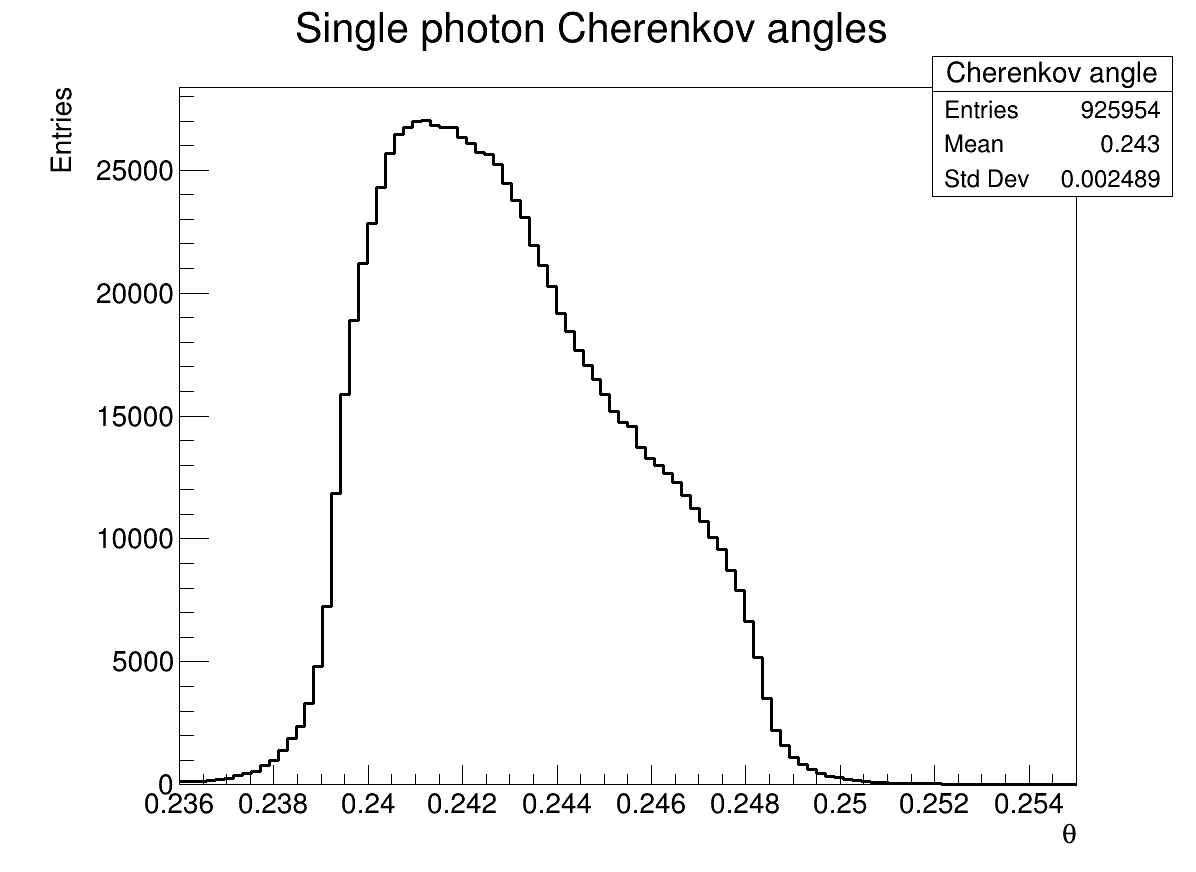
\includegraphics[width = 1.0\textwidth]{Plots/SinglePhotonCherenkovAngles_Barrel_Aerogel.png}
      \vspace{-0.75cm}
      \caption{Single photon uncertainty:\\ $\SI{2.5}{\milli\radian}$}
    \end{subfigure}%
    \begin{subfigure}{0.35\textwidth}
      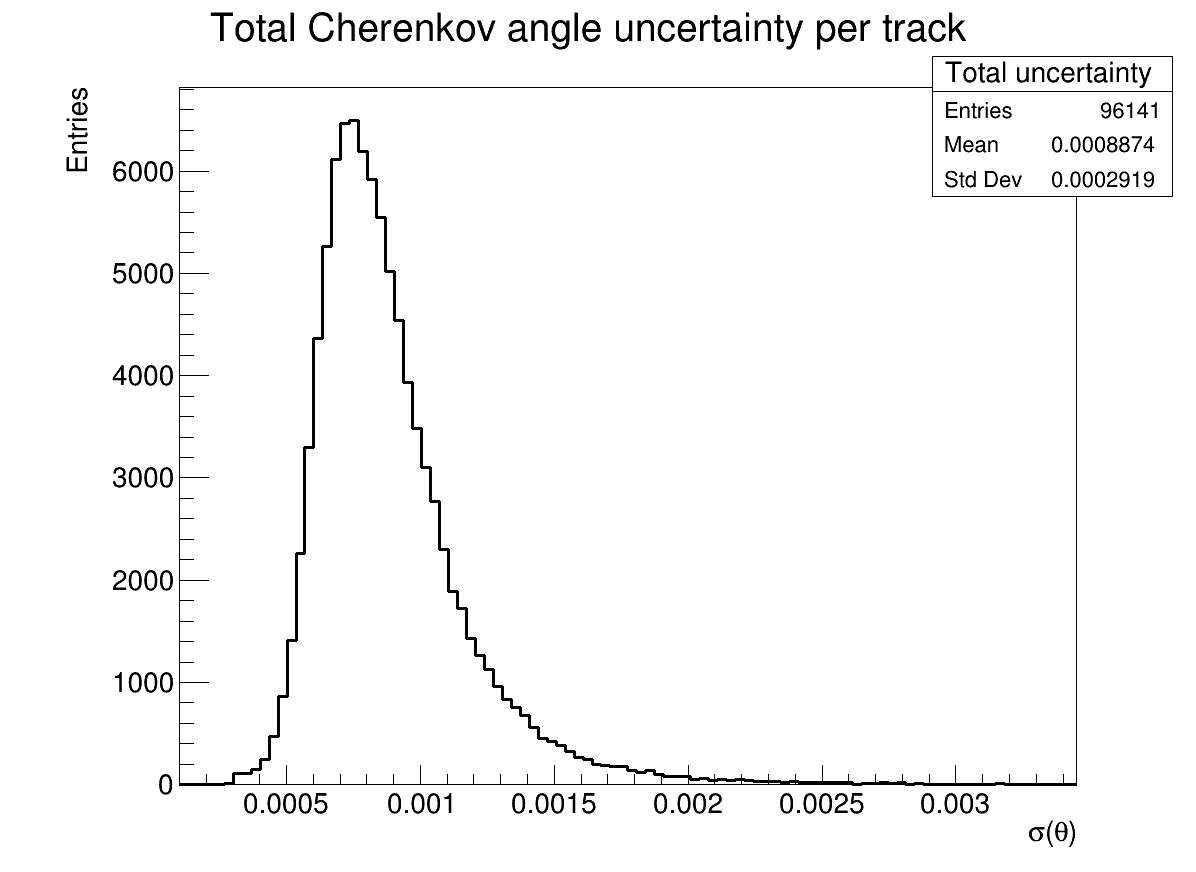
\includegraphics[width = 1.0\textwidth]{Plots/TotalCherenkovUncertainty_Barrel_Aerogel.png}
      \vspace{-0.75cm}
      \caption{Total uncertainty:\\ $\SI{0.9}{\milli\radian}$}
    \end{subfigure}
    \vspace{-0.1cm}
    \caption{Aerogel radiator performance averaged over all barrel cells}
  \end{figure}
\end{frame}

\section{Performance of optimised ARC}
\begin{frame}{Performance of optimised ARC}
  \begin{figure}
    \centering
    \vspace{-0.2cm}
    \begin{subfigure}{0.5\textwidth}
      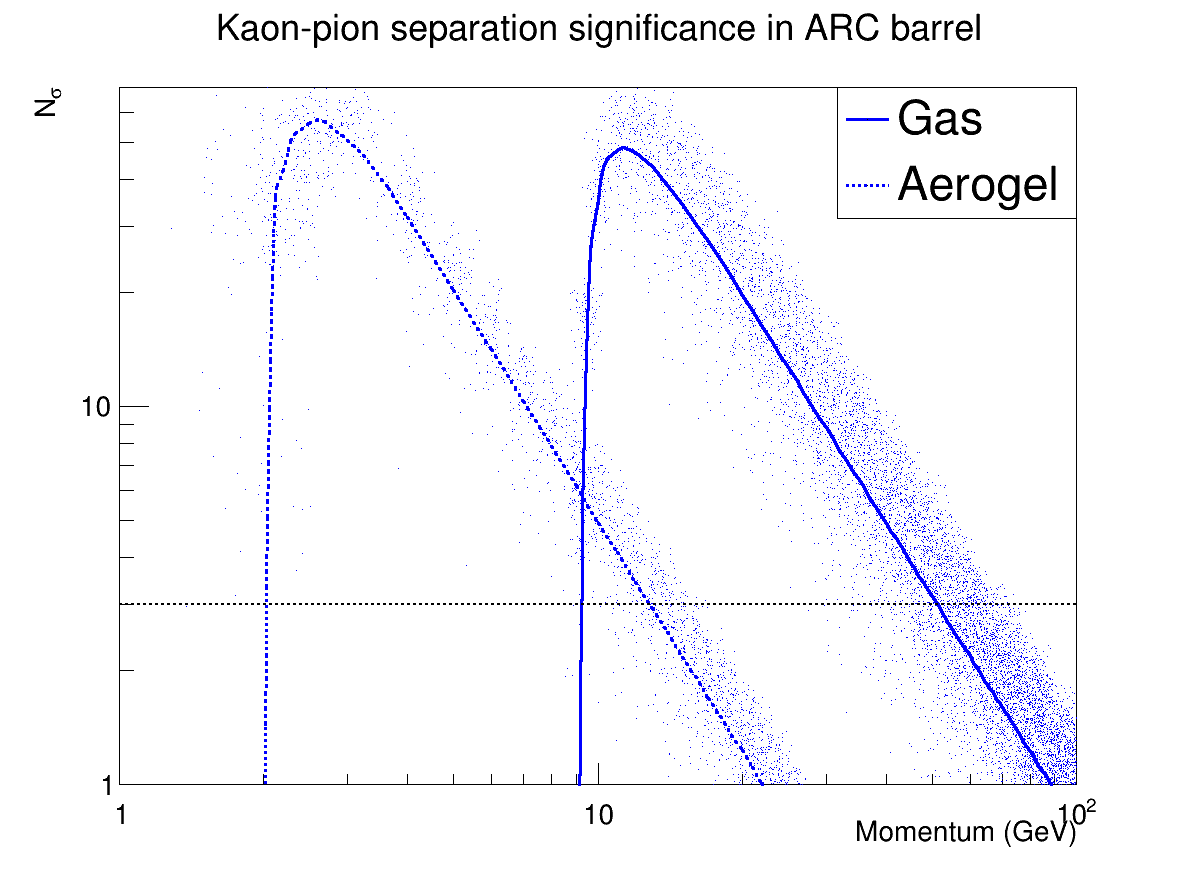
\includegraphics[width = 1.0\textwidth]{Plots/Significance_Scatter_PionKaon.png}
    \end{subfigure}%
    \begin{subfigure}{0.5\textwidth}
      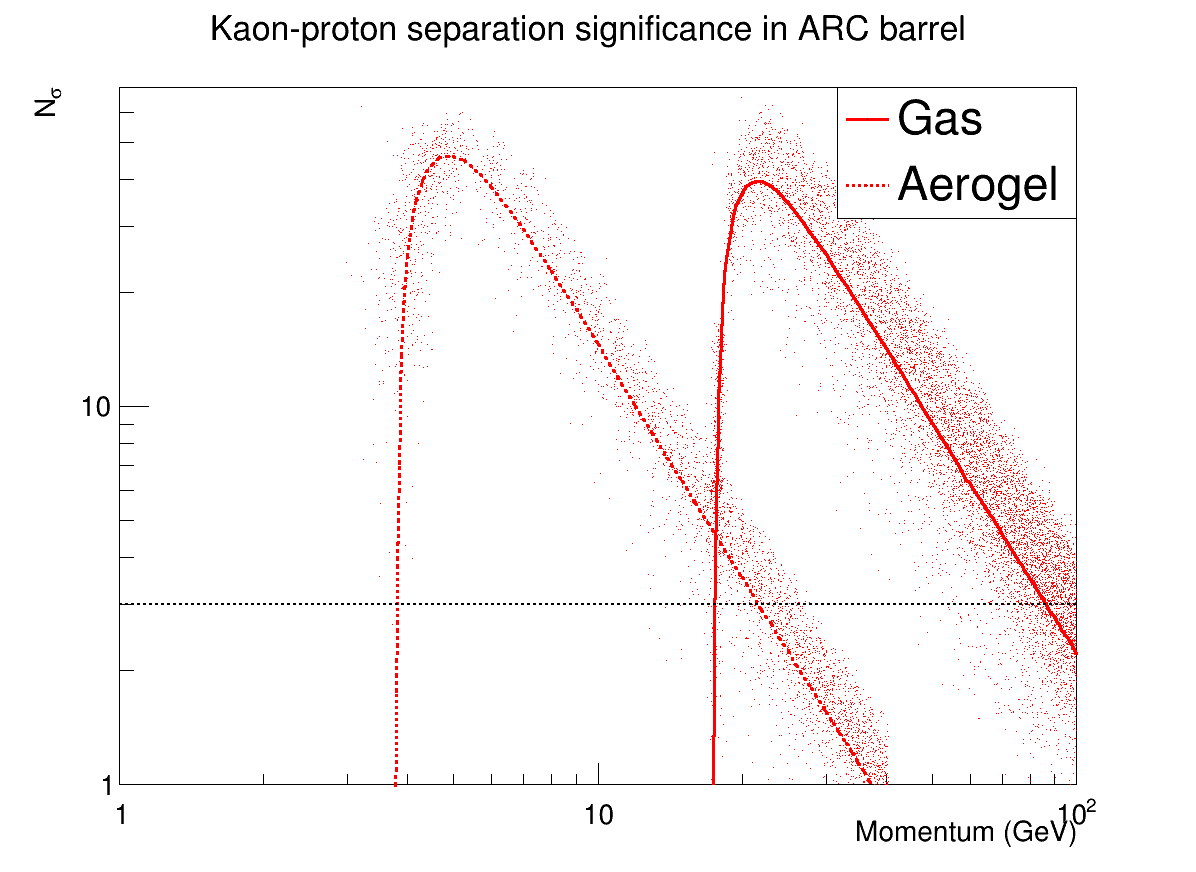
\includegraphics[width = 1.0\textwidth]{Plots/Significance_Scatter_ProtonKaon.png}
    \end{subfigure}
    \vspace{-0.4cm}
    \caption{Separation significance per track for $\pi$-$K$ (left) and $p$-$K$ (right)}
  \end{figure}
  \vspace{-0.4cm}
  \begin{itemize}
    \setlength\itemsep{0.0em}
    \item{Gas (aerogel) provides over $3\sigma$ pion-kaon separation in the range $10$-$\SI{50}{\giga\eV}$ ($2$-$\SI{10}{\giga\eV}$)}
    \begin{itemize}
      \item{Improved from earlier studies due to gaining some space for more radiator by no longer pressurising, as well as optimisation of the layout}
      \item{Effect of magnetic field not yet included in these studies}
    \end{itemize}
    \item{Combined, the aerogel and gas ensure excellent PID performance over the whole range of interest to flavour physics}
  \end{itemize}
\end{frame}

\section{Summary and next steps}
\begin{frame}{Summary and next steps}
  \begin{itemize}
    \setlength\itemsep{1.0em}
    \item{ARC is a low mass and compact cellular PID detector designed to occupy minimum space ($\SI{20}{\centi\meter}$ in the radial dimension) in a $4\pi$ detector at an $e^+e^-$ collider such as FCC-ee}
    \item{We have developed an optimised layout that should achieve a $3\sigma$ kaon-pion separation in the range $2$-$\SI{50}{\giga\eV}$}
    \begin{itemize}
      \item{Our studies focus mainly on flavour physics at the $Z$-pole}
    \end{itemize}
    \item{ARC will allow us to fully exploit the full range of flavour physics potential at future $e^+e^-$ colliders}
    \begin{itemize}
      \item{Will enhance the capabilities in Higgs, $WW$ and top physics}
    \end{itemize}
    \item{Next steps will include completing the optimisation, including magnetic field effects, and R\&D on photodetectors}
  \end{itemize}
  \begin{center}
    \huge Thanks for your attention!
  \end{center}
\end{frame}

\begin{frame}{Backup: Estimated material budget breakdown}
  \begin{center}
    Units of radiation length $X/X_0$
    \begin{tabular}{lcc}
        \hline
        Detector component                           & Pressurised & Non-pressurised \\
        \hline
        Vessel walls                                 & $5\%$                         & $1\%$ \\
        Photosensor array/electronics                & $1\%$                         & $1\%$ \\
        Cooling plate ($\SI{3}{\milli\meter}$ CF)    & $1\%$                         & $1\%$ \\
        Aerogel ($n = 1.03$)                         & $1\%$                         & $0.5\%$ \\
        C$_4$F$_{10}$ gas                              & $1\%$                         & $0.5\%$ \\
        Focusing mirror                              & $1\%$                         & $1\%$ \\
        \hline
        Total                                        & $10\%$                        & $5\%$ \\
        \hline
    \end{tabular}
  \end{center}
\end{frame}

\begin{frame}{Backup: Technical details about minimisation}
  \setlength\itemsep{1.0em}
  \begin{itemize}
    \item{$f(\vec{x})$ is not easily to calculate analytically}
    \item{Approximate by simulating a large number of charged tracks}
    \item{Finite number of photons $\implies f(\vec{x})$ is not differentiable}
    \begin{itemize}
      \item{Cannot be minimised using conventional methods (Minuit, etc)}
    \end{itemize}
    \item{I have experimented with a new type of minimisation algorithms: Stochastic optimisation}
    \begin{itemize}
      \item{\href{https://en.wikipedia.org/wiki/Differential_evolution}{Differential evolution}}
      \item{Start with a population of possible solutions, form new solutions by combining (mutating) existing solutions}
      \item{Advantage: Doesn't require initial guess, robust against functions that a not continuous, noisy, change over time, etc}
      \item{Disadvantage: No way to tell if optimal solution has been found, so it requires many iterations}
    \end{itemize}
  \end{itemize}
\end{frame}

\begin{frame}{Backup: Optimised mirror curvature and mirror position}
  \begin{figure}
    \centering
    \vspace{-0.2cm}
    \begin{subfigure}{0.5\textwidth}
      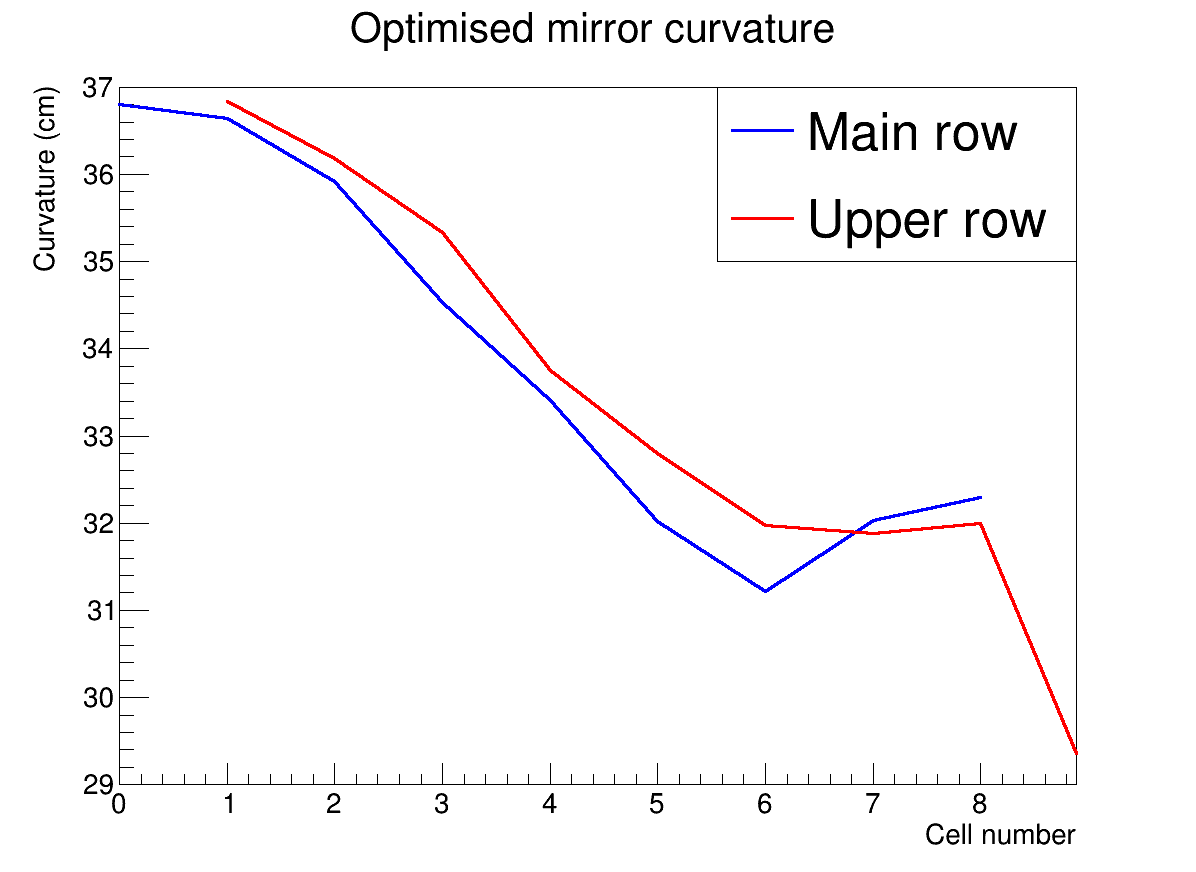
\includegraphics[width = 1.0\textwidth]{Plots/OptimisedMirrorCurvature.png}
      \caption{Mirror curvature}
    \end{subfigure}%
    \begin{subfigure}{0.5\textwidth}
      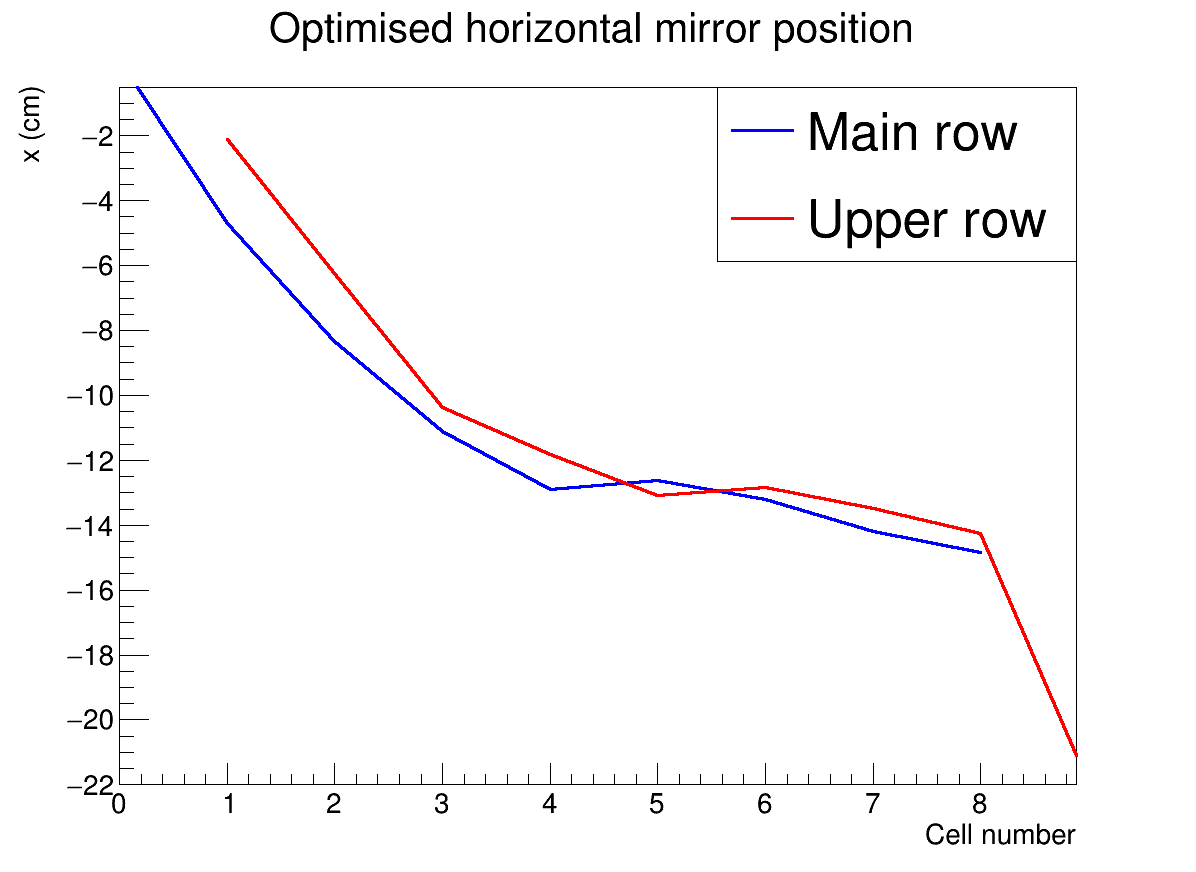
\includegraphics[width = 1.0\textwidth]{Plots/OptimisedMirrorX.png}
      \caption{Mirror position}
    \end{subfigure}
    \caption{Optimised mirror parameters for barrel cells}
  \end{figure}
\end{frame}

\begin{frame}{Backup: Optimised detector position and detector tilt angle}
  \begin{figure}
    \centering
    \vspace{-0.2cm}
    \begin{subfigure}{0.5\textwidth}
      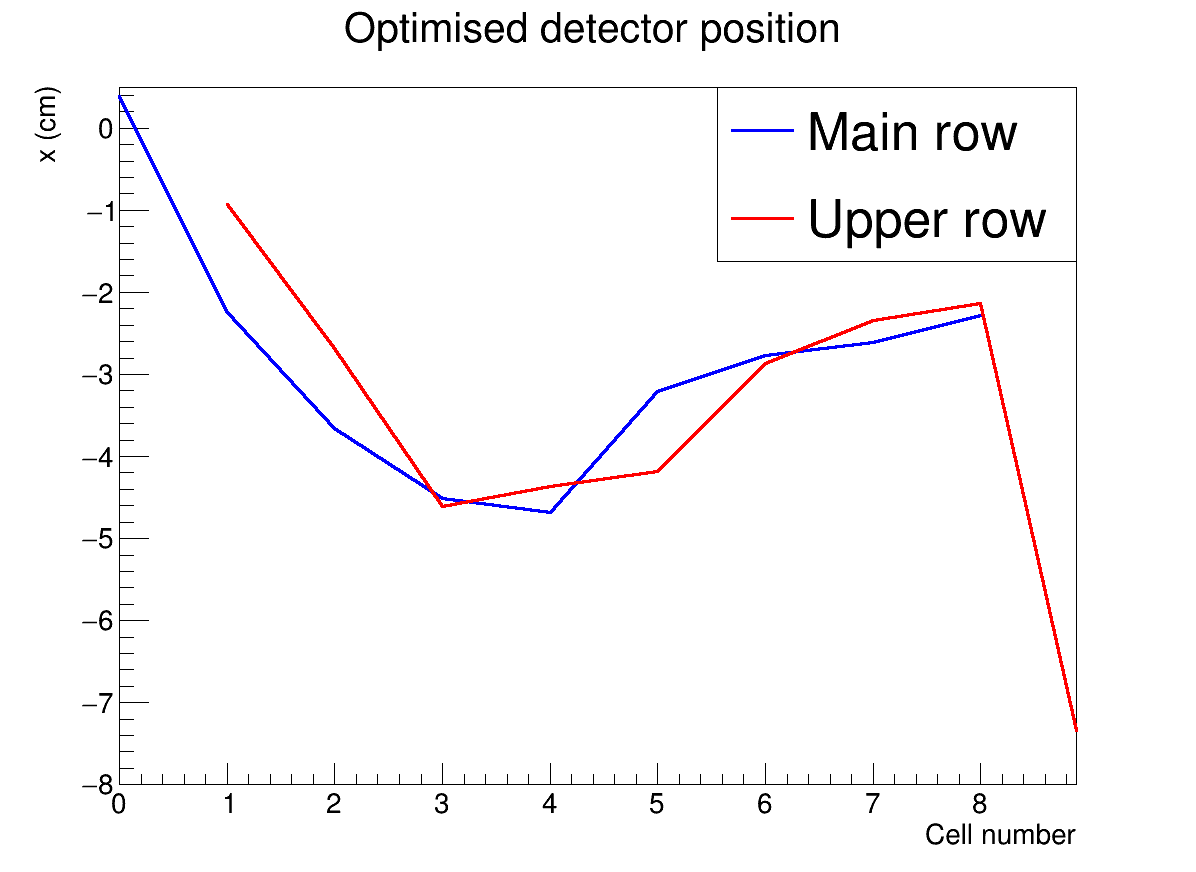
\includegraphics[width = 1.0\textwidth]{Plots/OptimisedDetPosition.png}
      \caption{Detector position}
    \end{subfigure}%
    \begin{subfigure}{0.5\textwidth}
      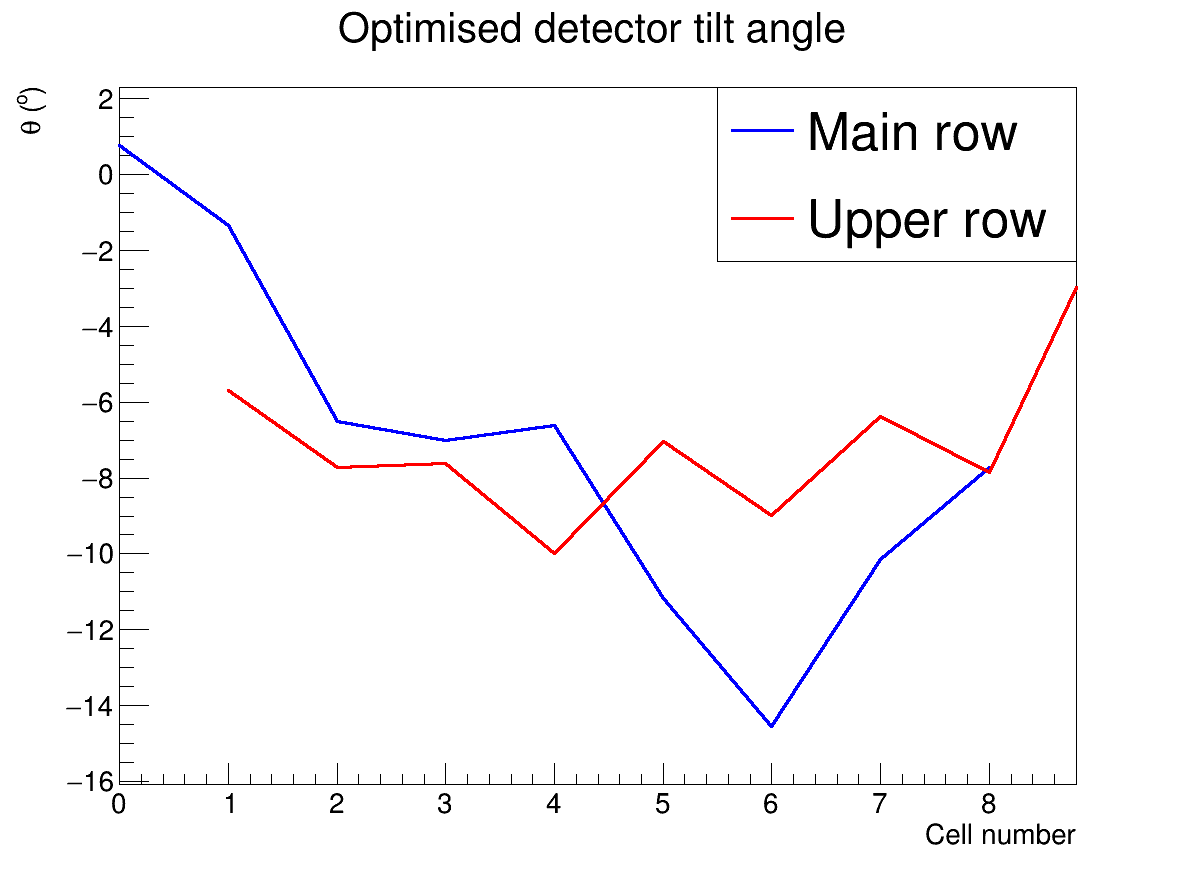
\includegraphics[width = 1.0\textwidth]{Plots/OptimisedDetTilt.png}
      \caption{Detector tilt angle}
    \end{subfigure}
    \caption{Optimised detector parameters for barrel cells}
  \end{figure}
\end{frame}

\end{document}